%%%%%%%%%%%%%%%%%%%%%%%%%%%%%%%%%%%%%%%%%
% University/School Laboratory Report
% LaTeX Template
% Version 3.1 (25/3/14)
%
% This template has been downloaded from:
% http://www.LaTeXTemplates.com
%
% Original author:
% Linux and Unix Users Group at Virginia Tech Wiki 
% (https://vtluug.org/wiki/Example_LaTeX_chem_lab_report)
%
% License:
% CC BY-NC-SA 3.0 (http://creativecommons.org/licenses/by-nc-sa/3.0/)
%
%%%%%%%%%%%%%%%%%%%%%%%%%%%%%%%%%%%%%%%%%

%----------------------------------------------------------------------------------------
%	PACKAGES AND DOCUMENT CONFIGURATIONS
%----------------------------------------------------------------------------------------

\documentclass[11pt,a4paper]{article}
\usepackage[utf8]{inputenc}
\usepackage[english,polish]{babel}
%\usepackage[T1]{fontenc}
\usepackage{polski}
\usepackage{amsfonts}
\usepackage[left=3cm,right=3cm,top=3cm,bottom=3cm]{geometry}
\usepackage{siunitx} % Provides the \SI{}{} and \si{} command for typesetting SI units
\usepackage{graphicx} % Required for the inclusion of images
\usepackage{natbib} % Required to change bibliography style to APA
\usepackage{amsmath} % Required for some math elements
\usepackage{epstopdf}
\usepackage[colorlinks=false,urlcolor=blue,citecolor=green]{hyperref}
\usepackage{fancyhdr}
\usepackage{lastpage}
\usepackage{array}
\usepackage{hhline}
\usepackage{svg}
\usepackage{multirow}
\usepackage{enumerate}%[I], numerki, [(a)]
\usepackage{float}
\usepackage{placeins}

%Figure numbering
\usepackage{chngcntr}
\counterwithin{figure}{section}
\counterwithin{equation}{section}

\newcommand*{\captionsource}[2]{%
  \caption[{#1}]{%
    #1%
    \\\hspace{\linewidth}%
    \textbf{Źródło:} #2%
  }%
}

\AtBeginDocument{
	\renewcommand{\tablename}{Tabela}
	\renewcommand{\figurename}{Rys.}
}

%tabelki
\usepackage{tabularx}
\newcolumntype{A}{>{\centering\arraybackslash}X}
\newcolumntype{B}{>{\centering\arraybackslash} m{0.4\textwidth} }

\setlength\parindent{0pt} % Removes all indentation from paragraphs

\renewcommand{\labelenumi}{\alph{enumi}.} % Make numbering in the enumerate environment by letter rather than number (e.g. section 6)

%\usepackage{times} % Uncomment to use the Times New Roman font

\title{\textbf{Model helikoptera}} % Title

\author{Marcin Kowalczyk \\ Maciej Cebula \\ Daniel Rubak} % Author name

\date{Kraków, 2017} % Date for the report

\begin{document}

\maketitle % Insert the title, author and date

\begin{center}
\begin{tabular}{l r}
Data wykonania: & 19 grudzień, 2017 \\ % Date the experiment was performed
Przedmiot: & Laboratorium Problemowe 2 \\
Prowadzący: & Dawid Knapik % Instructor/supervisor
\end{tabular}
\end{center}

\clearpage
\tableofcontents
\clearpage

\section{Wstęp}
\label{sec:wstep}
\subsection{Założenia}
Celem projektu było zaprojektowanie układu regulacji dla przybliżonego modelu helikoptera przedstawionego na rysunku \ref {heli_model}. Zaproponowany regulator powinien zapewnić stabilizację układu w zadanym położeniu oraz umożliwić śledzenie zadanej trajektorii. 
\subsection{Opis obiektu}
Do zmiany pozycji obiektu wykorzystywane były dwa niezależnie działające śmigła, zamontowane w dwóch prostopadłych osiach. Układ regulacji działa na zasadzie generowania momentu sił, pochodzących od obracających się śmigieł, w celu zniwelowania momentów wytworzonych przez siłę grawitacji oraz siłę odśrodkową. Moment siły wytwarzany przez silnik jest zależny od współczynnika wypełnienia sygnału PWM podawanego na niego. Tachoprądnice dołączone do każdego z silników oraz enkodery inkrementalne zamontowane w osiach obrotu  zapewniają pomiar orientacji obiektu i prędkości obrotowych silników prądu stałego. Połączenie wszystkich czujników z komputerem, na którym zainstalowano środowisko \textit{Matlab/Simulink}, poprzez kartę pomiarową, umożliwiło sterowanie całym procesem z poziomu \textit{Simulink-a}. W początkowej fazie projektu zdecydowano się wykonać układ sterowania dla helikoptera z zablokowaną osią pionową. 


\begin{figure}[h!]
	\centering
	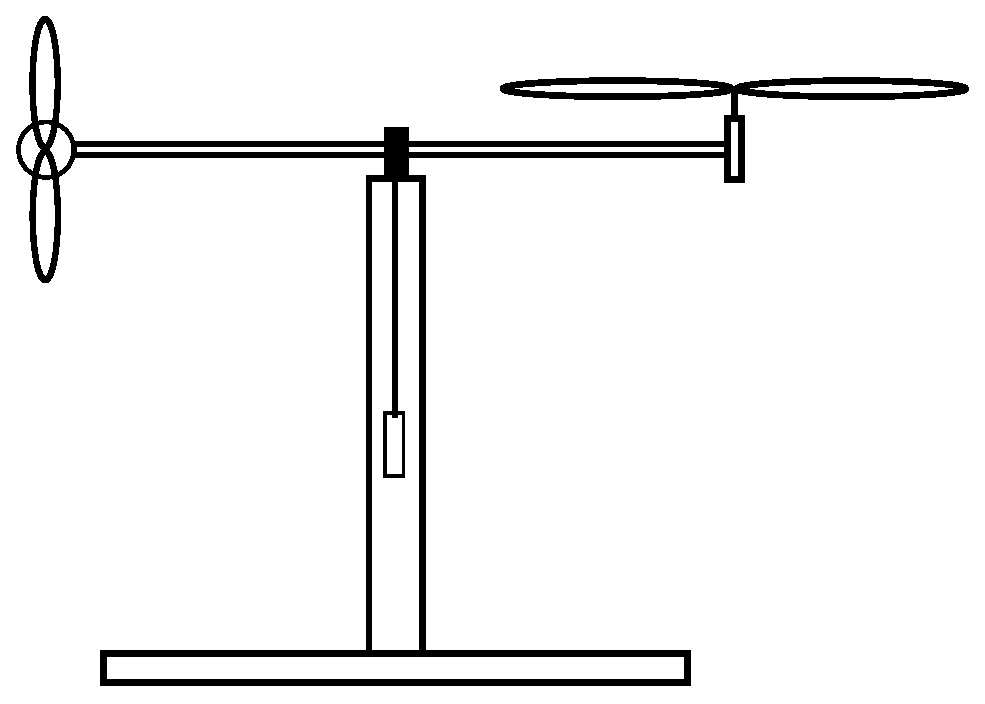
\includegraphics[scale = 0.4]{Figures/model_helikoptera.eps}
	\caption		
	{Helikopter - schemat obiektu sterowania}
	\label{heli_model}
\end{figure} 
Do symulacji, obliczeń numerycznych i generowania kodu wykorzystano programy \textit{Matlab} i \textit{Simulink}, które wykonywały cały algorytm sterujący w czasie rzeczywistym. \'Co więcej, środowisko to umożliwia zmianę parametrów układu sterowania (np. pozycji zadanej) w trakcie działania systemu oraz łatwy sposób archiwizacji i wizualizacji danych pomiarowych.

\FloatBarrier
\section{Model matematyczny}
\label{sec:modelmatematyczny}
Wykorzystano następujący model matematyczny układu dla osi poziomej:
\begin{equation}
\begin{aligned}
J_v \frac{d^2\alpha_v}{dt^2} &= -f_v\frac{d\alpha_v}{dt}+a\cdot sin(\alpha_v-\alpha_{v0})+M_v(\omega_v)\\
I_v\frac{d\omega_v}{dt} &= u_v - H_v^{-1}(\omega_v)
\end{aligned}
\label{eq:model_vertical}
\end{equation}
\noindent gdzie:\newline
\(\alpha_v\) jest kątem obrotu w płaszczyźnie pionowej,\newline
\(J_v\) jest momentem bezwładności względem osi obrotu w płaszczyźnie pionowej,\newline
\(f_v\) jest współczynnikiem tarcia lepkiego,\newline
\(a\) jest momentem sił grawitacji,\newline
\(\alpha_{v0}\) jest kątem równowagi układu w płaszczyźnie pionowej,\newline
\(I_v\) jest momentem bezwładności dużego śmigła,\newline
\(H_v^{-1}(\omega_v)\) jest charakterystyką statyczną układu silnik-śmigło dla silnika głównego,\newline
\(\omega_v\) jest prędkością obrotową silnika głównego,\newline
\(M_v(\omega_v)\) jest momentem sił generowanym przez silnik główny,\newline
\(u_v\) jest współczynnikiem wypełniania sygnału PWM dla silnika głównego.
\paragraph*{}
Dla osi pionowej wykorzystano następujący model matematyczny układu:
\begin{equation}
\begin{aligned}
J_h \frac{d^2\alpha_h}{dt^2} &= -f_h\frac{d\alpha_h}{dt}+M_h(\omega_h)\\
I_h\frac{d\omega_h}{dt} &= u_h - H_h^{-1}(\omega_h)
\end{aligned}
\label{eq:model_horizontal}
\end{equation}
\noindent gdzie:\newline
\(\alpha_h\) jest kątem obrotu w płaszczyźnie poziomej,\newline
\(J_h\) jest momentem bezwładności względem osi obrotu w płaszczyźnie poziomej,\newline
\(f_h\) jest współczynnikiem tarcia lepkiego,\newline
\(I_h\) jest momentem bezwładności małego śmigła,\newline
\(H_h^{-1}(\omega_h)\) jest charakterystyką statyczną układu silnik-śmigło dla silnika bocznego,\newline
\(\omega_h\) jest prędkością obrotową silnika bocznego,\newline
\(M_h(\omega_h)\) jest momentem sił generowanym przez silnik boczny,\newline
\(u_h\) jest współczynnikiem wypełniania sygnału PWM dla silnika bocznego.
\paragraph*{}
Przyjęto, że wielkości \(M_v(\omega_v)\), \(M_h(\omega_h)\), \(H_v^{-1}(\omega_v)\) i \(H_h^{-1}(\omega_h)\) są wielomianami piątego stopnia. Równania różniczkowe \eqref{eq:model_vertical} i \eqref{eq:model_horizontal} są więc równaniami nieliniowymi.

Równania \eqref{eq:model_vertical} i \eqref{eq:model_horizontal} przekształcono do postaci równań stanu. Dla równań \eqref{eq:model_vertical} mają one następującą postać:
\begin{equation}
\begin{aligned}
\dot x_1 &= x_2\\
\dot x_2 &= -\frac{f_v}{J_v}x_2+\frac{a}{J_v}\sin (\alpha_v-\alpha_{v0})+\frac{M_v(\omega_v)}{J_v}\\
\dot x_3 &= \frac{u_v}{I_v}-\frac{H_v^{-1}(\omega_v)}{I_v}
\end{aligned}
\label{eq:ss_vertical}
\end{equation}

Natomiast dla równań \eqref{eq:model_horizontal} mają następującą postać:
\begin{equation}
\begin{aligned}
\dot x_1 &= x_2\\
\dot x_2 &= -\frac{f_h}{J_h}x_2+\frac{M_h(\omega_h)}{J_h}\\
\dot x_3 &= \frac{u_h}{I_h}-\frac{H_h^{-1}(\omega_h)}{I_h}
\end{aligned}
\end{equation}

Opisany w tym rozdziale model dla osi poziomej został zaimplementowany w programie \textit{Simulink}. Schemat blokowy realizujący ten model przedstawiono na rysunku \ref{fig:Model_vertical}.

\begin{figure}[H]
	\centering
	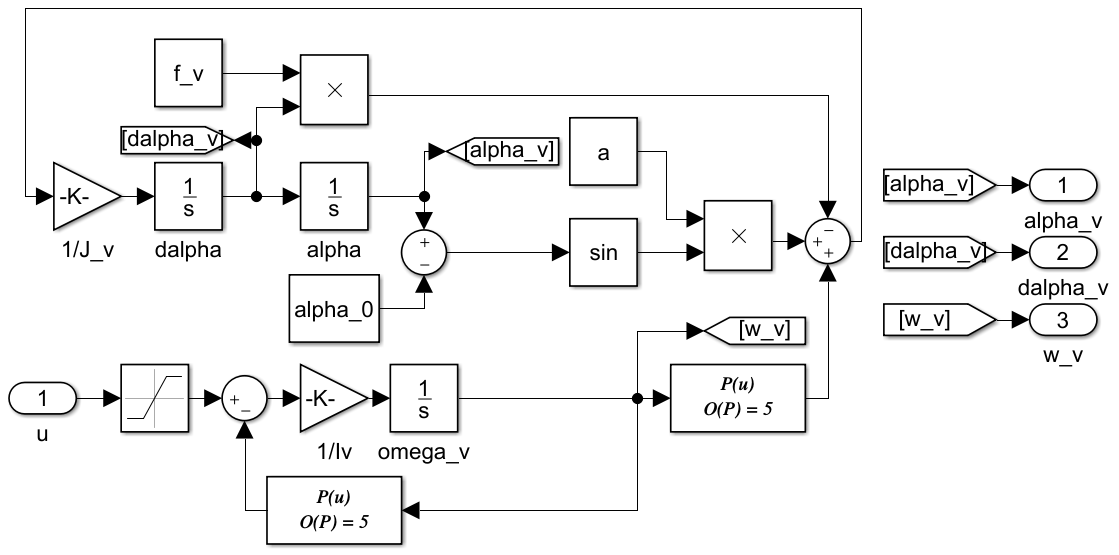
\includegraphics[width=5.9in]{Figures/Model_vertical.png}
	\caption{Model układu dla osi poziomej w programie \textit{Simulink}.}
	\label{fig:Model_vertical}
\end{figure}

\section{Identyfikacja}
\label{sec:identyfikacja}
Zagadnienie identyfikacji modeli nieliniowych jest bardzo często zagadnieniem problematycznym. Dla modeli liniowych wystarczy zazwyczaj wykorzystać metodę najmniejszych kwadratów. Dla modelu nieliniowego metoda ta daje na ogół obciążoną estymację parametrów, a rozwiązanie zadania może być niejednoznaczne. Oprócz tego zadanie to jest skomplikowane pod względem numerycznym, gdyż rozwiązywania nieliniowych równań różniczkowych jest złożone obliczeniowo. Aby ułatwić identyfikację należy zdekomponować ją na znacznie prostsze zadania. Dzięki temu identyfikacja modelu nieliniowego sprowadza się do wykonania kilkudziesięciu pomiarów oraz odpowiednich przekształceń algebraicznych.

\subsection{Prędkość kątowa z prądnicy tachometrycznej}
W pierwszej kolejności konieczne było przeliczenie napięcia z prądnicy tachometrycznej na prędkość kątową w radianach na sekundę. W tym celu wykorzystano dostępną dokumentację oraz zebrane pomiary. Dla danej wartości współczynnika wypełnienia PWM odczytywano multimetrem napięcie na wyprowadzeniach z prądnicy tachometrycznej oraz wartość wyświetlaną w \textit{Simulink}. W dokumentacji sprawdzono jak należy przeliczyć napięcie prądnicy tachometrycznej na prędkość kątową. Punkty pomiarowe następnie aproksymowano wielomianem pierwszego stopnia. Wyniki zostały zaprezentowane na rysunku \ref{fig:char_V_U}.

\begin{figure}[H]
	\centering
	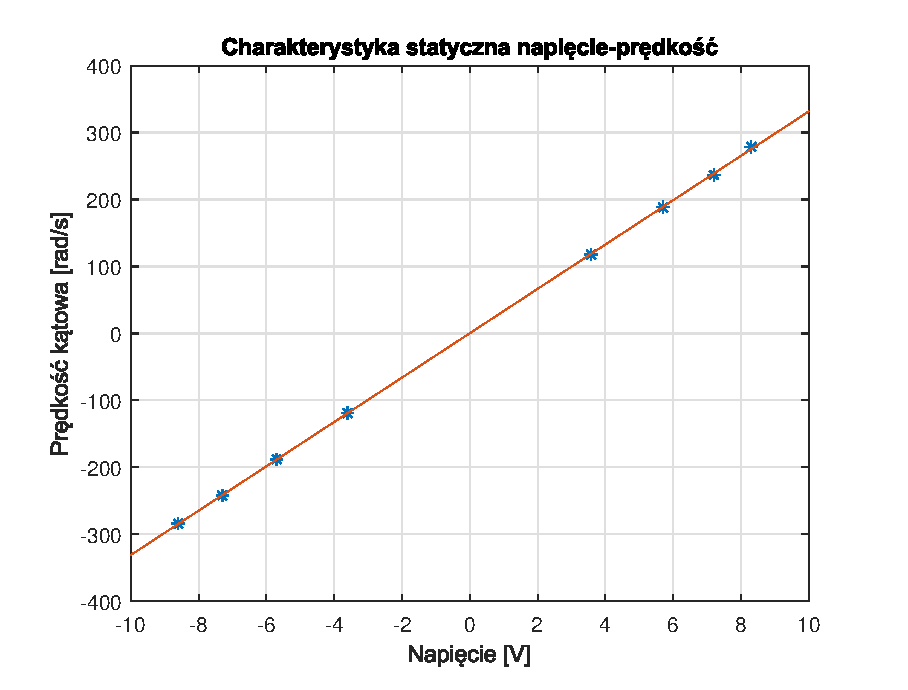
\includegraphics[width=4in]{Figures/char_V_U.eps}
	\caption{Charakterystyka statyczna prędkości kątowej od odczytu z czujnika.}
	\label{fig:char_V_U}
\end{figure}

Otrzymano wzór \eqref{eq:V_Vs} opisujący przeliczenie wielkości odczytanej w \textit{Simulink} na prędkość kątową w radianach na sekundę.
\begin{equation}
V = \frac{2000\pi}{0.52\cdot 60}(0.1644V_S+0.0019)
\label{eq:V_Vs}
\end{equation}
\noindent gdzie:\newline
\(V_S\) jest wartością odczytaną w \textit{Simulink},\newline
\(V\) jest prędkością kątową w radianach na sekundę.

\subsection{Moment niewyważenia}
Wykonano badanie momentu niewyważenia, który powodował,że kiedy na układ nie działały żadne dodatkowe siły, to nie znajdował się on w pozycji poziomej. Rozpoczęto od zgrubnego wyznaczenia kąta równowagi w płaszczyźnie pionowej. W tym celu użyto elektronicznej "poziomicy" w postaci telefonu komórkowego. Wyznaczony kąt miał wartość:
\begin{equation}
\alpha_{v0} = -0.491 \ rad
\end{equation}
Następnie wykorzystano równanie \eqref{eq:moment_niewywazenia} do wyznaczenia zależności momentu niewyważenia od kąta nachylenia (parametru \(a\)).
\begin{equation}
J_v \frac{d^2\alpha_v}{dt^2} = -f_v\frac{d\alpha_v}{dt}+a\cdot \sin(\alpha_v-\alpha_{v0})+M_v(\omega_v)
\label{eq:moment_niewywazenia}
\end{equation}
W pewnej odległości \(l\) od osi obrotu przyłożono siłę (pochodzącą od zawieszonych ciężarków), której moment był przeciwny do momentu niewyważenia. Wagę ciężarków dobrano tak, by powstały moment równoważył niewyważenie dla kąta \(\alpha_v=0 \ rad \). Kąt ten nie zmienia się, a więc jego pochodne są równe \(0\). Można więc zapisać równania \eqref{eq:M_zew} opisujące równowagę sił w tej sytuacji.
\begin{equation}
\begin{aligned}
M_{zew} &= -a\cdot \sin(\alpha_v-\alpha_{v0})\\
M_{zew} &= lmg\cos(\alpha_v)
\end{aligned}
\label{eq:M_zew}
\end{equation}
\noindent gdzie:\newline
\(a\) jest maksymalnym momentem sił niewyważenia,\newline
\(\alpha_v\) jest kątem obrotu w płaszczyźnie pionowej,\newline
\(\alpha_{v0}\) jest kątem równowagi układu w płaszczyźnie pionowej,\newline
\(M_{zew}\) jest przyłożonym momentem sił,\newline
\(l\) jest odległością od osi obrotu do punktu przyłożenia zewnętrznej siły,\newline
\(m\) jest łączną masą przyłożonych ciężarków,\newline
\(g\) jest przyspieszeniem ziemskim.
\paragraph*{}
Opisane parametry miały następujące wartości:
\begin{equation}
\begin{aligned}
\alpha_v &= 0\\
\alpha_{v0} &= -0.491\\
l &= 0.26\si{m}\\
m &= 0.06\si{kg}\\
g &= 9.81\si{m/s^2}
\end{aligned}
\end{equation}
Podstawiając wartości powyższych parametrów do wzorów \eqref{eq:M_zew} wyznaczono następującą wartość współczynnika momentu niewyważenia:
\begin{equation}
a = -0.3068\si{Nm}
\end{equation}

\subsection{Moment siły generowany przez silnik główny}
Następnie konieczne było wyznaczenie momentu siły generowanego przez śmigło przymocowane do silnika głównego. W tym celu podawano różne wartości współczynnika wypełnienia PWM na silnik. Po ustaleniu się prędkości obrotowej zawieszano ciężarki w pewnej odległości od osi obrotu tak, aby przyłożony zewnętrzny moment siły równoważył moment siły wygenerowany przez silnik oraz moment niewyważenia dla kąta \(\alpha_v=0\). W tym celu ponownie wykorzystano równanie \eqref{eq:moment_niewywazenia}. Kąt nachylenia nie zmieniał się, a więc pochodne kąta nachylenia po czasie wynosiły \(0\). Wzór ten sprowadzał się więc do zależności opisanej wzorem
\begin{equation}
\begin{aligned}
M_v(\omega_v) &= -a\cdot \sin(\alpha_v-\alpha_{v0})-M_{zew}\\
M_{zew} &= lmg\cos(\alpha_v)
\end{aligned}
\label{eq:moment_sily_glowny}
\end{equation}
\noindent gdzie:\newline
\(a\) jest maksymalnym momentem sił niewyważenia,\newline
\(\alpha_v\) jest kątem obrotu w płaszczyźnie pionowej,\newline
\(\alpha_{v0}\) jest kątem równowagi układu w płaszczyźnie pionowej,\newline
\(M_{zew}\) jest przyłożonym momentem sił,\newline
\(M_v(\omega_v)\) jest momentem siły generowanym przez silnik główny,\newline
\(\omega_v\) jest prędkością obrotową silnika głównego,\newline
\(l\) jest odległością od osi obrotu do punktu przyłożenia zewnętrznej siły,\newline
\(m\) jest łączną masą przyłożonych ciężarków,\newline
\(g\) jest przyspieszeniem ziemskim.
\paragraph*{}
Zależność momentu siły nośnej od prędkości kątowej postanowiono aproksymować wielomianem piątego stopnia. Na wykresie \ref{fig:char_M_V} kolorem czerwonym zaznaczone zostały wyznaczone punkty pomiarowe, natomiast kolorem niebieskim funkcja aproksymująca (wielomian).

\begin{figure}[H]
	\centering
	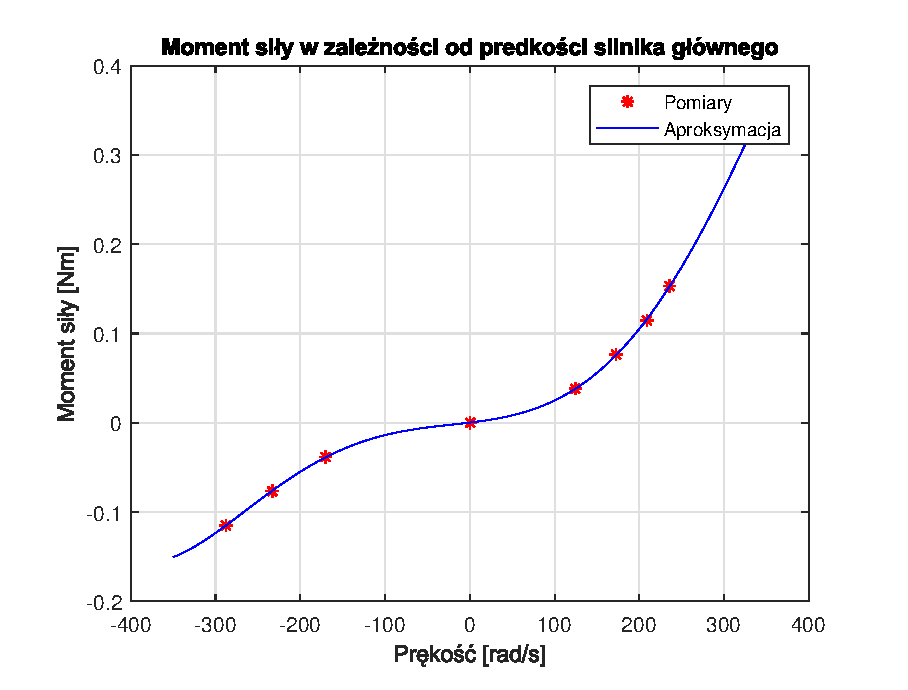
\includegraphics[width=4in]{Figures/char_M_V.eps}
	\caption{Charakterystyka statyczna momentu siły nośnej od prędkości obrotowej silnika.}
	\label{fig:char_M_V}
\end{figure}

Badana zależność wyraża się następującym wzorem:
\begin{equation}
\begin{aligned}
M_v(\omega_v) &= -2.5146\cdot 10^{-14}\omega_v^5+2.9593\cdot 10^{-12}\omega_v^4+8.1312\cdot 10^{-9}\omega_v^3\\ & \quad +5.0407\cdot 10^{-7}\omega_v^2+1.1510\cdot 10^{-4}\omega_v+2.7833\cdot 10^{-4}
\end{aligned}
\end{equation}

\subsection{Zależność oporów ruchu od prędkości obrotowej śmigła głównego}
Kolejnym krokiem procesu identyfikacji było badanie wpływu prędkości obrotowej silnika na napięcie podawane na silnik. Większa prędkość obrotowa powoduje większe opory, przez co mniejsze napięcie podawane jest na silnik. Opisuje to równanie \eqref{eq:domega_v}.
\begin{equation}
I_v\frac{d\omega_v}{dt} = u_v - H_v^{-1}(\omega_v)
\label{eq:domega_v}
\end{equation}
\noindent gdzie:\newline
\(I_v\) jest momentem bezwładności dużego śmigła,\newline
\(H_v^{-1}(\omega_v)\) jest charakterystyką statyczną układu silnik-śmigło dla silnika głównego,\newline
\(\omega_v\) jest prędkością obrotową silnika głównego,\newline
\(u_v\) jest współczynnikiem wypełniania sygnału PWM dla silnika głównego.
\paragraph*{}
Pomiary wykonywane są dla ustalonej prędkości obrotowej silnika, więc jej pochodne po czasie są równe \(0\). Stąd powyższe równie przyjmuje następującą postać:
\begin{equation}
H_v^{-1}(\omega_v) = u_v
\end{equation}
Zależność oporów ruchu śmigła od prędkości kątowej postanowiono aproksymować wielomianem piątego stopnia. Na wykresie \ref{fig:char_U_V} kolorem czerwonym zaznaczone zostały wyznaczone punkty pomiarowe, natomiast kolorem niebieskim funkcja aproksymująca (wielomian).

\begin{figure}[H]
	\centering
	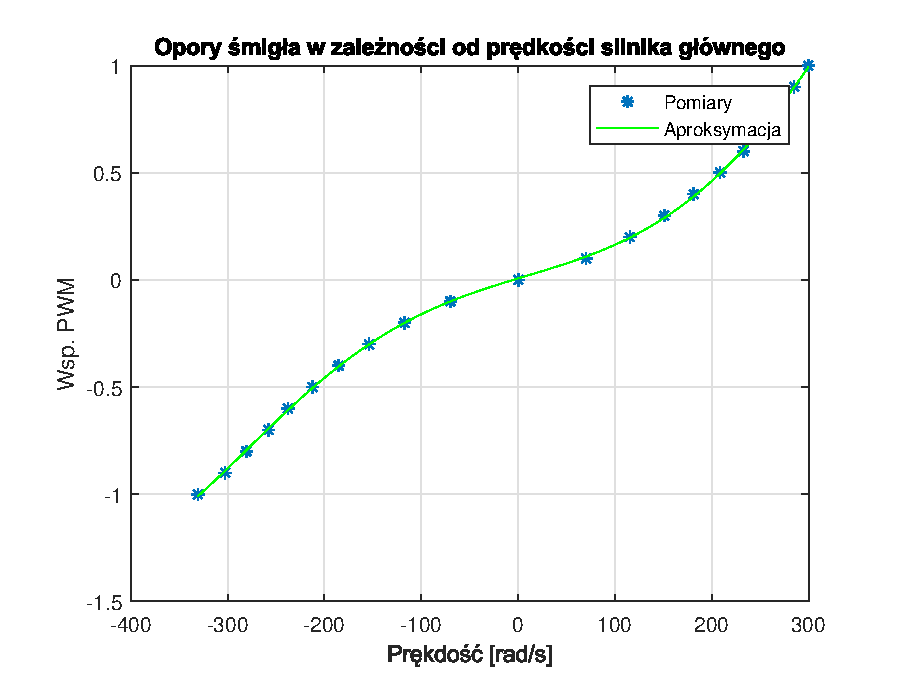
\includegraphics[width=4in]{Figures/char_U_V.eps}
	\caption{Charakterystyka statyczna oporów ruchu śmigła od prędkości obrotowej silnika.}
	\label{fig:char_U_V}
\end{figure}

Badana zależność wyraża się następującym wzorem:
\begin{equation}
\begin{aligned}
H_v^{-1}(\omega_v) &= -7.4418\cdot 10^{-14}\omega_v^5+1.3631\cdot 10^{-11}\omega_v^4+2.6232\cdot 10^{-8}\omega_v^3\\ & \quad -6.6054\cdot 10^{-7}\omega_v^2+0.0014\omega_v+0.0072
\end{aligned}
\end{equation}

\subsection{Parametry modelu układu silnik DC - śmigło główne}
Następnie przeprowadzono identyfikację parametrów równania \eqref{eq:uklad_silnik_smiglo_v}.
\begin{equation}
I_v\frac{d\omega_v}{dt} = u_v - H_v^{-1}(\omega_v)
\label{eq:uklad_silnik_smiglo_v}
\end{equation}
Funkcja \(H_v^{-1}(\omega_v)\) została już zidentyfikowana. Należy więc dobrać tylko wartość momentu bezwładności dużego śmigła (\(I_v\)). W tym celu zarejestrowano odpowiedź prędkości obrotowej śmigła na skok wartości współczynnika wypełniania sygnału PWM podawanego na silnik. Następnie z wykorzystaniem funkcji \textit{lsqnonlin} programu \textit{MATLAB} znaleziono taką wartość tego parametru, która minimalizuje błąd średniokwadratowy odpowiedzi modelu względem zarejestrowanego przebiegu. Do rozwiązywania równania różniczkowego \eqref{eq:uklad_silnik_smiglo_v} w procesie optymalizacji użyto funkcji \textit{ode45}. Na rysunku \ref{fig:ident_I_v} kolorem niebieskim przedstawiono zarejestrowany przebieg, a kolorem czerwonym odpowiedź aproksymowanego modelu.

\begin{figure}[H]
	\centering
	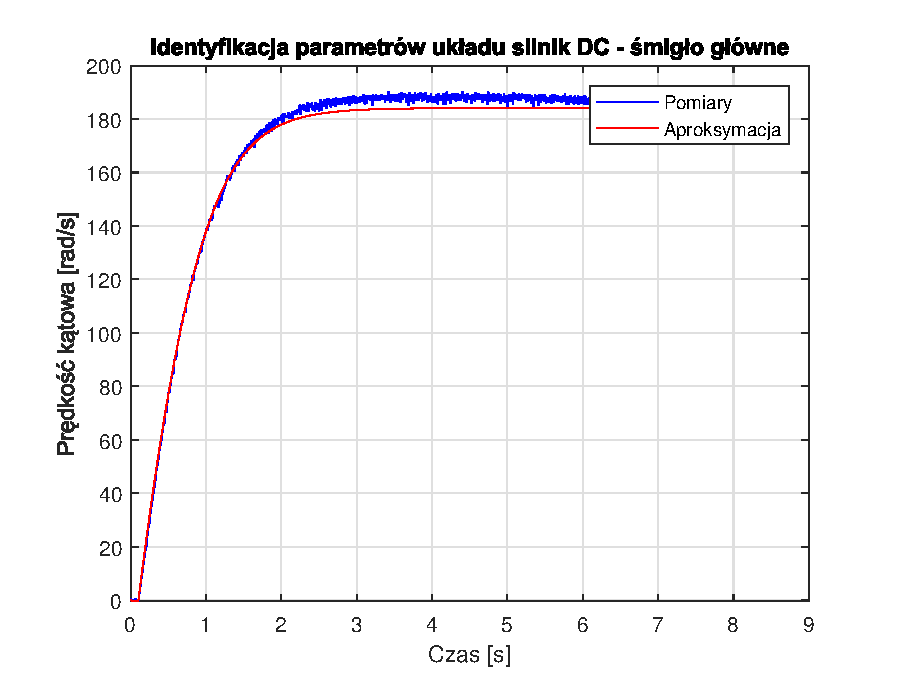
\includegraphics[width=4in]{Figures/ident_I_v.eps}
	\caption{Porównanie odpowiedzi zarejestrowanej i aproksymowanego modelu.}
	\label{fig:ident_I_v}
\end{figure}

Wyznaczony parametr miał następującą wartość:
\begin{equation}
I_v = 0.0017\si{kg.m^2}
\end{equation}

\subsection{Moment bezwładności układu dla osi poziomej}
Ostatnimi koniecznymi do zbadania parametrami dla układu w płaszczyźnie pionowej były jego moment bezwładności, współczynnik tarcia lepkiego oraz dokładna wartość kąta równowagi układu. Wielkości te zostały wyznaczone na podstawie równania \eqref{eq:ident_J_v}.
\begin{equation}
J_v \frac{d^2\alpha_v}{dt^2} = -f_v\frac{d\alpha_v}{dt}+a\cdot sin(\alpha_v-\alpha_{v0})+M_v(\omega_v)
\label{eq:ident_J_v}
\end{equation}
Identyfikację tej części przeprowadzano wprowadzając układ w drgania wokół punktu równowagi. W trakcie eksperymentu silnik był wyłączony. Równanie \eqref{eq:ident_J_v} sprowadza się więc do postaci:
\begin{equation}
J_v \frac{d^2\alpha_v}{dt^2} = -f_v\frac{d\alpha_v}{dt}+a\cdot sin(\alpha_v-\alpha_{v0})
\end{equation}
Zapisano przebieg kąta wychylenia układu podczas eksperymentu. Następnie szukano parametrów \(J_v\), \(f_v\) oraz \(\alpha_{v0}\) takich, by minimalizowały średniokwadratowy wskaźnik jakości. Wykorzystano do tego funkcję \textit{lsqnonlin} programu \textit{MATLAB}. Na rysunku \ref{fig:ident_J_v} kolorem niebieskim przedstawiono zarejestrowany przebieg, a kolorem czerwonym odpowiedź aproksymowanego modelu.

\begin{figure}[H]
	\centering
	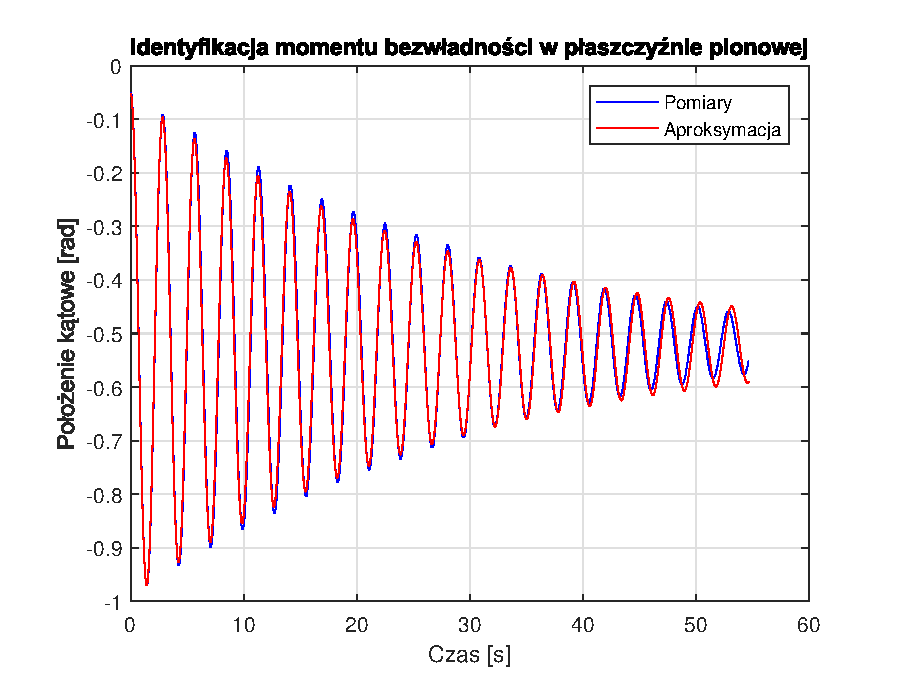
\includegraphics[width=4in]{Figures/ident_J_v.eps}
	\caption{Porównanie odpowiedzi zarejestrowanej i aproksymowanego modelu.}
	\label{fig:ident_J_v}
\end{figure}

W wyniku optymalizacji otrzymano następujące wartości poszukiwanych parametrów modelu:
\begin{equation}
\begin{aligned}
J_v &= 0.0604\si{kg.m^2}\\
f_v &= 0.0042\si{Nm.s}\\
\alpha_{v0} &= -0.5223
\end{aligned}
\end{equation}

\subsection{Zależność oporów ruchu od prędkości obrotowej śmigła bocznego}
Następnie zbadano wpływ prędkości obrotowej silnika na napięcie podawane na silnik dla osi pionowej. Podobnie jak dla osi poziomej, większa prędkość obrotowa powoduje większe opory, przez co mniejsze napięcie podawane jest na silnik. Opisuje to równanie \eqref{eq:domega_h}.
\begin{equation}
I_h\frac{d\omega_h}{dt} = u_h - H_h^{-1}(\omega_h)
\label{eq:domega_h}
\end{equation}
\noindent gdzie:\newline
\(I_h\) jest momentem bezwładności śmigła bocznego,\newline
\(H_h^{-1}(\omega_h)\) jest charakterystyką statyczną układu silnik-śmigło dla silnika bocznego,\newline
\(\omega_h\) jest prędkością obrotową silnika bocznego,\newline
\(u_h\) jest współczynnikiem wypełniania sygnału PWM dla silnika bocznego.
\paragraph*{}
Pomiary wykonano dla ustalonej prędkości obrotowej silnika, więc jej pochodne po czasie są równe \(0\). Stąd powyższe \eqref{eq:domega_h} przyjmuje następującą postać:
\begin{equation}
H_h^{-1}(\omega_h) = u_h
\end{equation}
Zależność oporów ruchu śmigła od prędkości kątowej postanowiono aproksymować wielomianem piątego stopnia. Na wykresie \ref{fig:char_U_V_az} kolorem czerwonym zaznaczone zostały wyznaczone punkty pomiarowe, natomiast kolorem niebieskim funkcja aproksymująca (wielomian).

\begin{figure}[H]
	\centering
	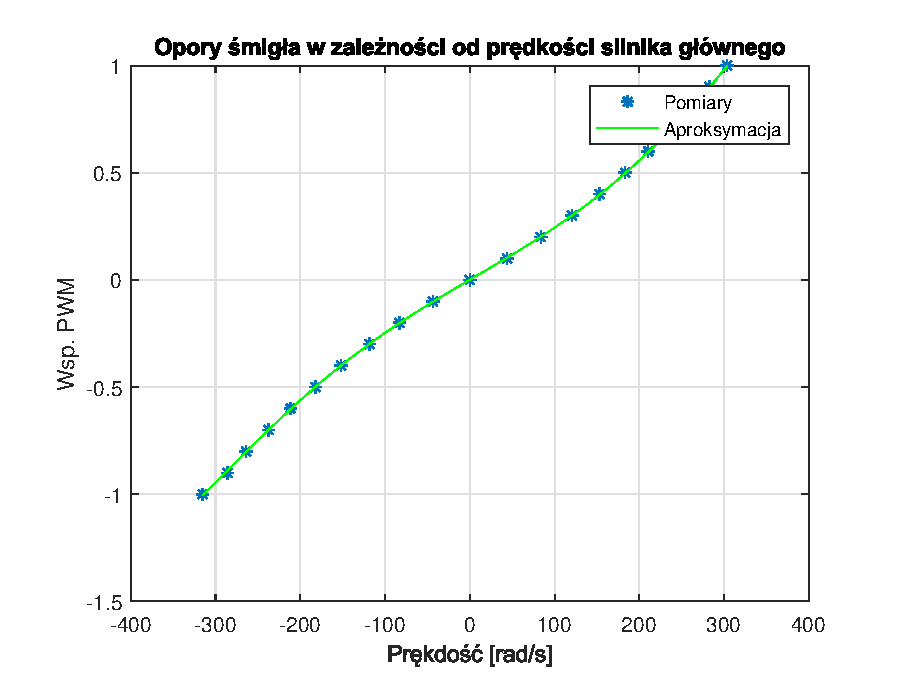
\includegraphics[width=4in]{Figures/char_U_V_az.eps}
	\caption{Charakterystyka statyczna oporów ruchu śmigła bocznego od prędkości obrotowej silnika.}
	\label{fig:char_U_V_az}
\end{figure}

Badana zależność wyraża się następującym wzorem:
\begin{equation}
\begin{aligned}
H_h^{-1}(\omega_h) &= -4.0004\cdot 10^{-14}\omega_h^5+5.1822\cdot 10^{-12}\omega_h^4+1.3426\cdot 10^{-8}\omega_h^3\\ & \quad -2.8251\cdot 10^{-7}\omega_h^2+0.0023\omega_h+6.8066\cdot 10^{-4}
\end{aligned}
\end{equation}

\subsection{Parametry modelu układu silnik DC - śmigło boczne}
Konieczne było przeprowadzenie identyfikacji parametrów równania \eqref{eq:uklad_silnik_smiglo_h}.
\begin{equation}
I_h\frac{d\omega_h}{dt} = u_h - H_h^{-1}(\omega_h)
\label{eq:uklad_silnik_smiglo_h}
\end{equation}
Funkcja \(H_h^{-1}(\omega_h)\) została zidentyfikowana w poprzednim podrozdziale. Należy więc dobrać wartość momentu bezwładności śmigła bocznego (\(I_h\)). W tym celu zarejestrowano odpowiedź prędkości obrotowej śmigła na skok wartości współczynnika wypełniania sygnału PWM podawanego na silnik. Następnie dla zarejestrowanego przebiegu użyto funkcję \textit{lsqnonlin} programu \textit{MATLAB}, by znaleźć taką wartość parametru \(I_h\), która minimalizuje błąd średniokwadratowy odpowiedzi modelu. Do rozwiązywania równania różniczkowego \eqref{eq:uklad_silnik_smiglo_h} w procesie optymalizacji użyto funkcji \textit{ode45}. Na rysunku \ref{fig:ident_I_h} kolorem niebieskim przedstawiono zarejestrowany przebieg, a kolorem czerwonym odpowiedź aproksymowanego modelu.

\begin{figure}[H]
	\centering
	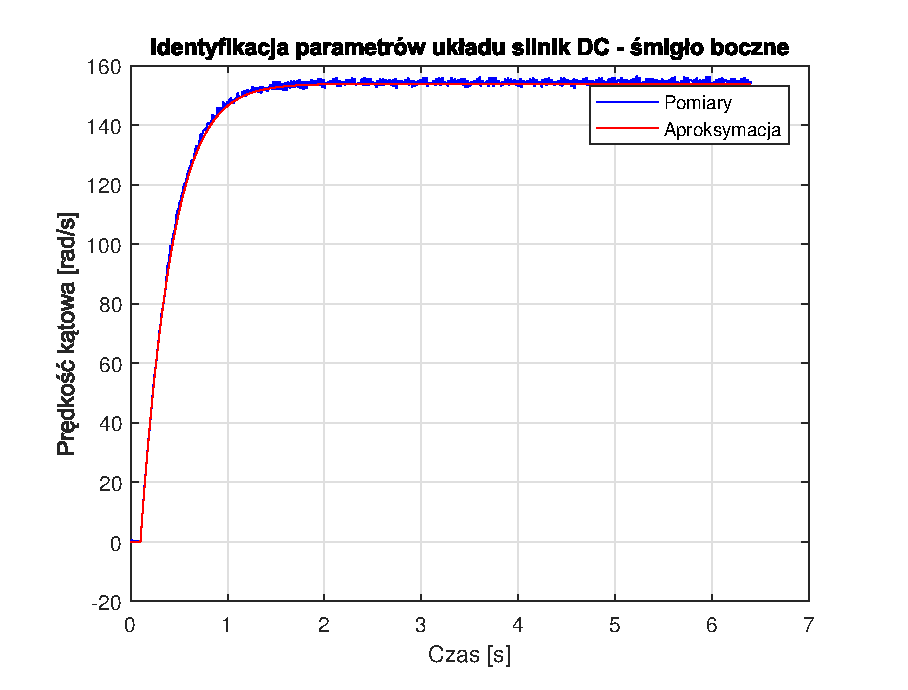
\includegraphics[width=4in]{Figures/ident_I_h.eps}
	\caption{Porównanie zapisanego przebiegu i odpowiedzi zidentyfikowanego modelu.}
	\label{fig:ident_I_h}
\end{figure}

Wyznaczony parametr miał następującą wartość:
\begin{equation}
I_h = 8.7148\cdot 10^{-4}\si{kg.m^2}
\end{equation}

\subsection{Moment siły generowany przez silnik boczny}
Przeprowadzono również eksperyment w celu wyznaczenia momentu siły generowanego przez śmigło boczne. W tym celu podawano różne wartości współczynnika wypełnienia PWM na silnik przy zablokowanym układzie. Po ustaleniu się prędkości obrotowej układ uwalniano i zapisywano przebiegi położenia kątowego i prędkości obrotowej silnika. W tym celu wykorzystano równanie \eqref{eq:moment_sily_boczny}.
\begin{equation}
J_h \frac{d^2\alpha_h}{dt^2} = -f_h\frac{d\alpha_h}{dt}+M_h(\omega_h)
\label{eq:moment_sily_boczny}
\end{equation}
\noindent gdzie:\newline
\(\alpha_h\) jest kątem obrotu w płaszczyźnie poziomej,\newline
\(J_h\) jest momentem bezwładności względem osi obrotu w płaszczyźnie poziomej,\newline
\(f_h\) jest współczynnikiem tarcia lepkiego,\newline
\(\omega_h\) jest prędkością obrotową silnika bocznego,\newline
\(M_h(\omega_h)\) jest momentem sił generowanym przez silnik boczny.
\paragraph*{}
W celu zmniejszenia ilości parametrów koniecznych do optymalizacji postanowiono obie strony równania podzielić przez \(J_h\). Otrzymane równanie poddano procesowi identyfikacji.Na wykresie \ref{fig:V_ident_J_h} przedstawiono prędkość obrotową silnika. Jest ona w przybliżeniu stała (pomijając szumy pomiarowe). Można więc założyć, że również moment wywołany tą prędkością jest stały. W związku z tym identyfikacja sprowadza się do znalezienia parametru \(f_v\) i stałego momentu siły.

\begin{figure}[H]
	\centering
	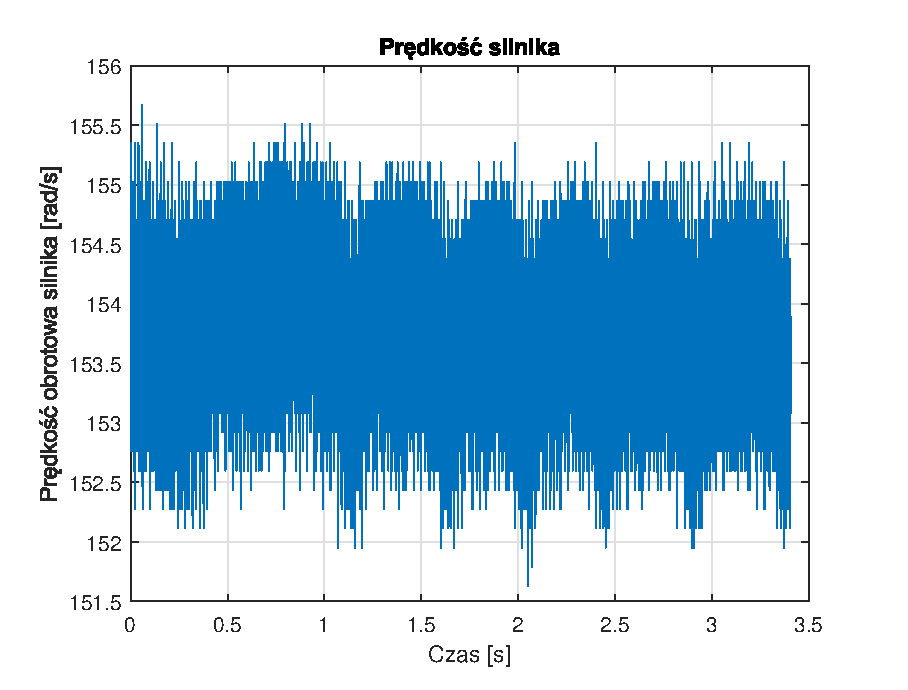
\includegraphics[width=4in]{Figures/V_ident_J_h.eps}
	\caption{Prędkość obrotowa silnika w trakcie eksperymentu.}
	\label{fig:V_ident_J_h}
\end{figure}

Dla zarejestrowanych przebiegów użyto funkcji \textit{lsqnonlin} programu \textit{MATLAB}, by znaleźć takie wartości współczynników, które minimalizują błąd średniokwadratowy odpowiedzi modelu. Do rozwiązywania równania różniczkowego \eqref{eq:moment_sily_boczny} w procesie optymalizacji użyto funkcji \textit{ode45}. Na rysunku \ref{fig:ident_J_h} kolorem niebieskim przedstawiono jeden z zarejestrowanych przebiegów, a kolorem czerwonym odpowiedź aproksymowanego modelu.

\begin{figure}[H]
	\centering
	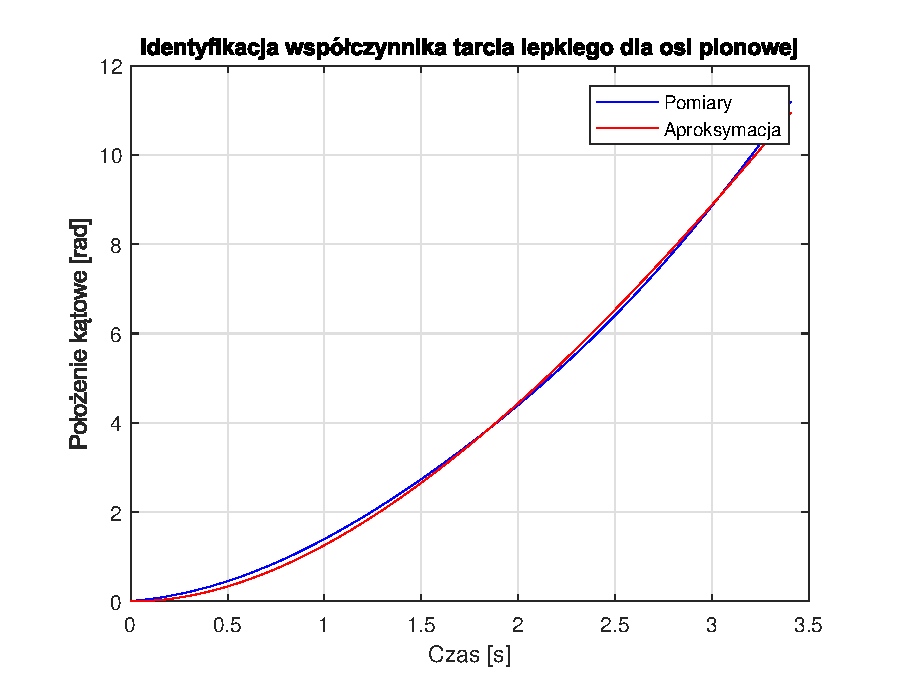
\includegraphics[width=4in]{Figures/ident_J_h.eps}
	\caption{Porównanie zarejestrowanej odpowiedzi z aproksymowanym modelem.}
	\label{fig:ident_J_h}
\end{figure}

Wyznaczony parametr \(f_h\) miał następującą wartość:
\begin{equation}
f_h = 0.0539
\end{equation}
Następnie zarejestrowano dane z eksperymentów, podczas których układ nie był zablokowany po podaniu skoku współczynnika wypełnienia sygnału PWM na silnik. Dane te znacznie lepiej nadają się do zidentyfikowania współczynników wielomianu \(M_h(\omega_h)\). Na wykresie \ref{fig:V_ident_M_h} przedstawiono przebieg prędkości obrotowej silnika podczas jednego z przeprowadzonych eksperymentów.

\begin{figure}[H]
	\centering
	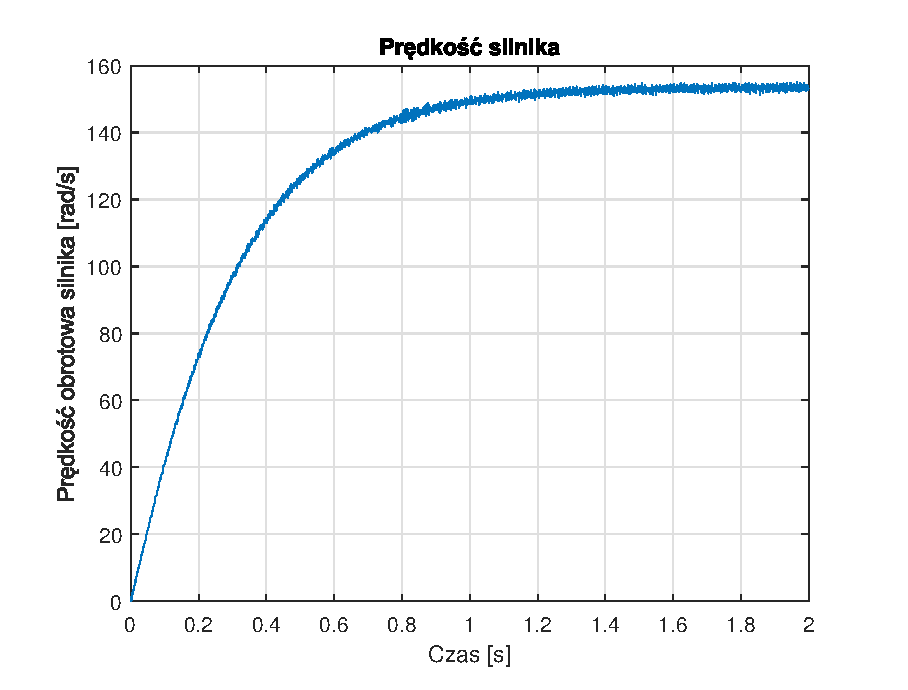
\includegraphics[width=4in]{Figures/V_ident_M_h.eps}
	\caption{Prędkość obrotowa silnika w trakcie eksperymentu.}
	\label{fig:V_ident_M_h}
\end{figure}

Za pomocą funkcji \textit{lsqnonlin} wyznaczono współczynniki wielomianu \(M_h(\omega_h)\), które minimalizowały średniokwadratowy wskaźnik jakości dla zarejestrowanych przebiegów. Na wykresach \ref{fig:ident_M_h_04} i \ref{fig:ident_M_h_-06} kolorem niebieskim oznaczono zarejestrowany przebieg, a kolorem czerwonym odpowiedź aproksymowanego modelu. Pierwszy z wykresów odpowiada skokowi współczynnika wypełnienia do wartości 0.4, natomiast drugi skokowi tej wielkości do -0.6 (silnik obracający się w przeciwną stronę).

\begin{figure}[H]
	\centering
	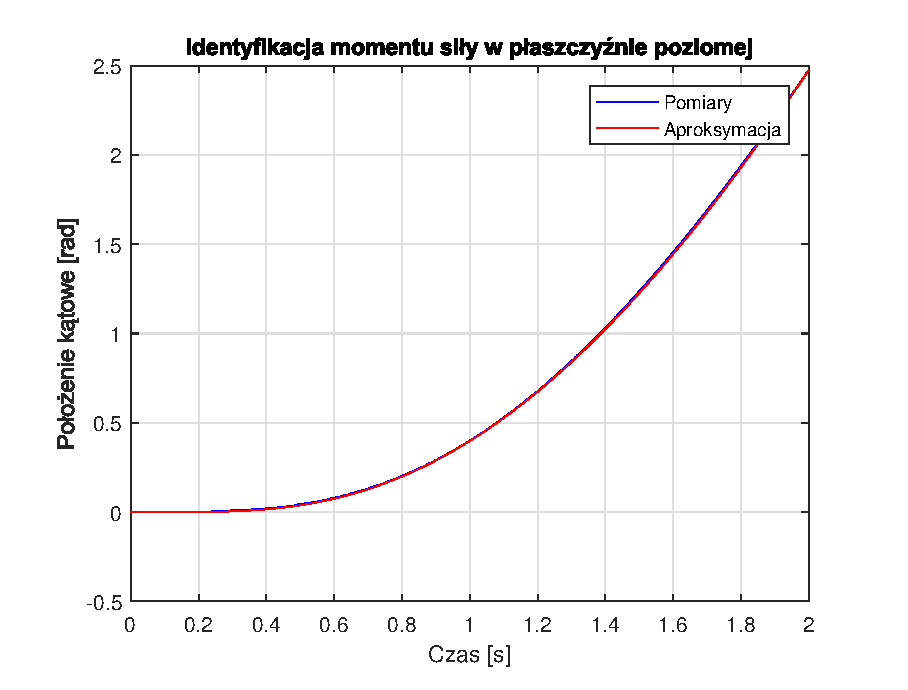
\includegraphics[width=4in]{Figures/ident_M_h_04.eps}
	\caption{Porównanie odpowiedzi dla współczynnika wypełnienia PWM równego \(0.4\).}
	\label{fig:ident_M_h_04}
\end{figure}

\begin{figure}[H]
	\centering
	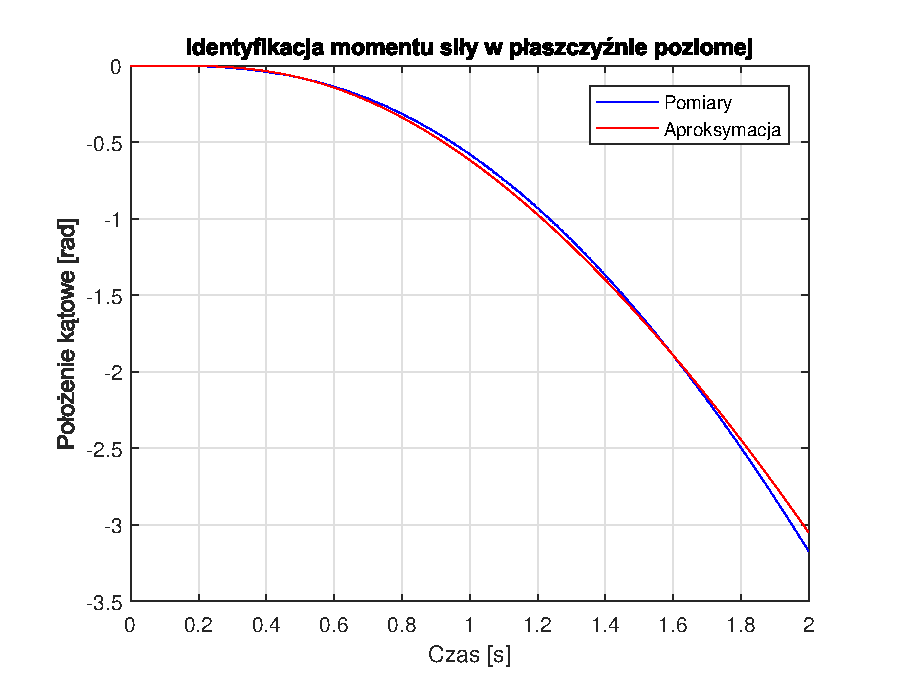
\includegraphics[width=4in]{Figures/ident_M_h_-06.eps}
	\caption{Porównanie odpowiedzi dla współczynnika wypełnienia PWM równego \(-0.6\).}
	\label{fig:ident_M_h_-06}
\end{figure}

Na rysunku \ref{fig:ident_M_h} przedstawiono wykres wyznaczonej funkcji momentu siły zależnej od prędkości obrotowej silnika bocznego \(M_h(\omega_h)\).

\begin{figure}[H]
	\centering
	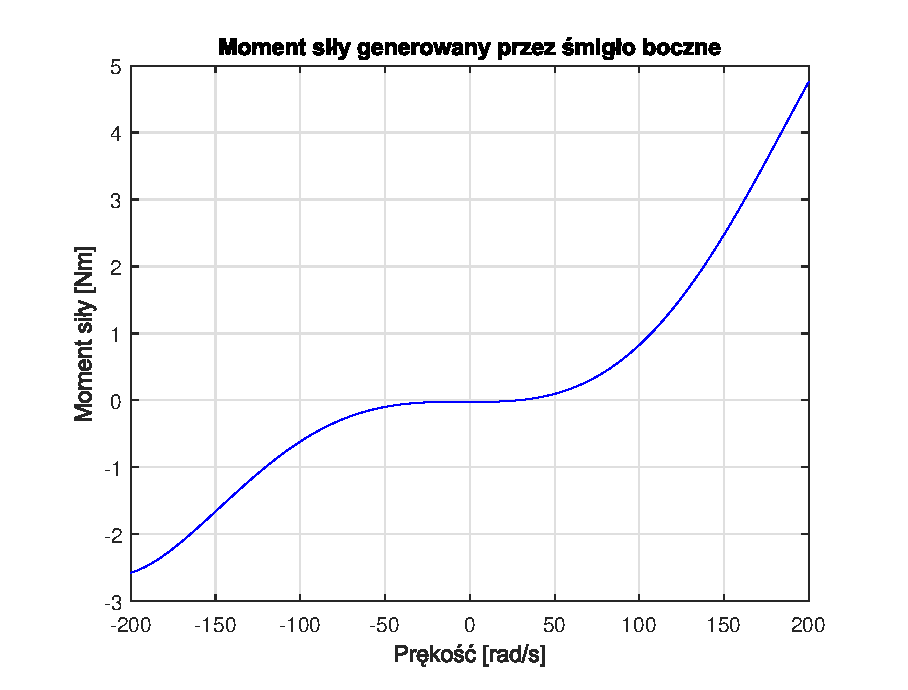
\includegraphics[width=4in]{Figures/ident_M_h.eps}
	\caption{Moment siły w zależności od prędkości obrotowej silnika bocznego.}
	\label{fig:ident_M_h}
\end{figure}

Powyższa funkcja opisana jest następującym wzorem:
\begin{equation}
\begin{aligned}
M_h(\omega_h) &= -8.8567\cdot 10^{-12}\omega_h^5+4.9851\cdot 10^{-10}\omega_h^4+8.1331\cdot 10^{-7}\omega_h^3\\ & \quad +7.9455\cdot 10^{-6}\omega_h^2-3.3890\cdot 10^{-5}\omega_h-0.0215
\end{aligned}
\end{equation}

\section{Punkt równowagi}
\label{sec:punktrownowagi}
W dalszej części pracy projektowano sterowanie układem z zablokowanym ruchem w płaszczyźnie poziomej. W tym celu konieczne było wyznaczenie zbioru punktów równowagi systemu. Punkt spełnia następujące równania:
\begin{equation}
\begin{aligned}
\dot x_1 &= 0\\
\dot x_2 &= 0\\
\dot x_3 &= 0
\end{aligned}
\end{equation}
A więc:
\begin{equation}
\begin{aligned}
0 &= x_2\\
0 &= -\frac{f_v}{J_v}x_2+\frac{a}{J_v}\sin (\alpha_v-\alpha_{v0})+\frac{M_v(\omega_v)}{J_v}\\
0 &= \frac{u_v}{I_v}-\frac{H_v^{-1}(\omega_v)}{I_v}
\end{aligned}
\label{eq:equilibrium_point}
\end{equation}
Z powyższych równań wynika, że w każdym punkcie równowagi prędkość kątowa układu \(x_2\) jest równa \(0\). Natomiast zmienne stanu \(x_1\) i \(x_2\) oraz sterowanie tworzą w przestrzeni trójwymiarowej pewien zbiór punktów równowagi. Dla przyjętych wartości \(x_1\) (położenie kątowe) wyznaczono takie wartości \(x_3\) i \(u\), że układ znajduje się w punkcie równowagi. W tym celu konieczne jest rozwiązanie równania \eqref{eq:equilibrium_x3} ze względu na \(x_3\).
\begin{equation}
M_v(\omega_v)+a\sin (\alpha_v-\alpha_{v0}) = 0
\label{eq:equilibrium_x3}
\end{equation}
Warto zauważyć, że w rozpatrywanym zakresie prędkości kątowej silnika funkcja \(M_v(\omega_v)\) jest ściśle monotonicznie rosnąca. Można to zauważyć na wykresie \ref{fig:char_M_V}. W związku z tym równanie \eqref{eq:equilibrium_x3} ma tylko jedno rozwiązanie. Sterowanie \(u\) w punkcie równowagi należy wyliczyć ze wzoru \eqref{eq:equilibrium_u}.
\begin{equation}
u_v = H_v^{-1}(\omega_v)
\label{eq:equilibrium_u}
\end{equation}
Wykres \ref{fig:e_p_3d} przedstawia wyznaczony zbiór punktów równowagi w przestrzeni trójwymiarowej.

\begin{figure}[H]
	\centering
	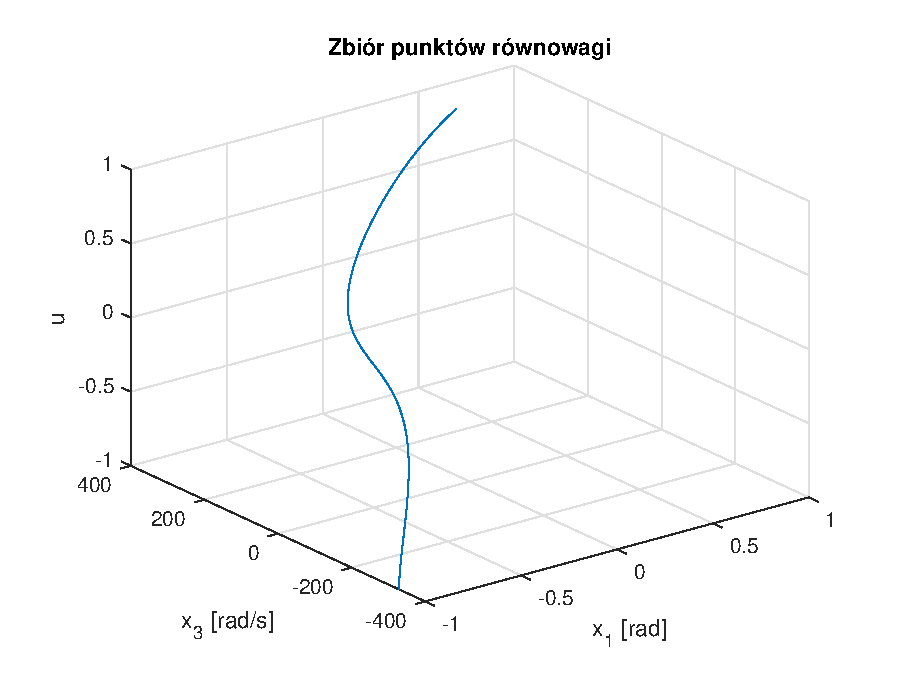
\includegraphics[width=4in]{Figures/e_p_3d.eps}
	\caption{Zbiór punktów równowagi układu.}
	\label{fig:e_p_3d}
\end{figure}

Rysunek \ref{fig:e_p_x1_x3} wyraża zależność prędkości kątowej silnika od położenia układu w punkcie równowagi, natomiast rysunek \ref{fig:e_p_x1_u} zależność współczynnika wypełnienia PWM od położenia układu w punkcie równowagi.

\begin{figure}[H]
	\centering
	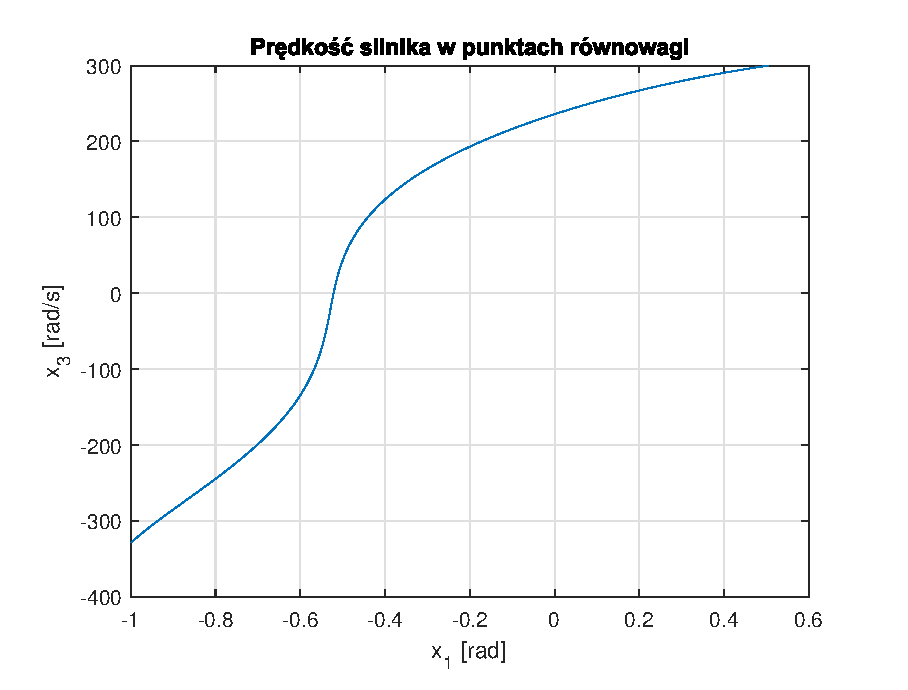
\includegraphics[width=4in]{Figures/e_p_x1_x3.eps}
	\caption{Zależność prędkości silnika od położenia układu w punkcie równowagi.}
	\label{fig:e_p_x1_x3}
\end{figure}

\begin{figure}[H]
	\centering
	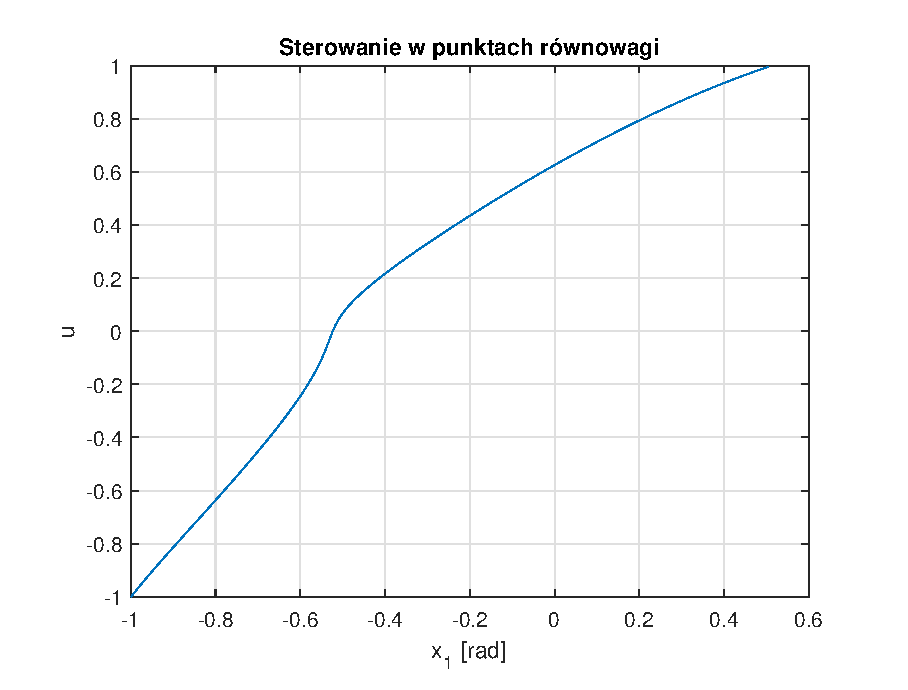
\includegraphics[width=4in]{Figures/e_p_x1_u.eps}
	\caption{Zależność sterowania od położenia układu w punkcie równowagi.}
	\label{fig:e_p_x1_u}
\end{figure}

\section{Linearyzacja}
\label{sec:linearyzacja}
W procesie projektowania układu sterowania konieczne było wyznaczenie modelu zlinearyzowanego w punkcie równowagi. Jest to model liniowy, który w otoczeniu punktu równowagi zachowuje się tak samo lub podobnie do modelu nieliniowego. Model linowy jest opisany równaniem różniczkowym \eqref{eq:linear}.
\begin{equation}
\begin{aligned}
\dot x &= Ax+Bu\\
y &= Cx+Du
\end{aligned}
\label{eq:linear}
\end{equation}
\noindent gdzie:\newline
\(x\) jest wektorem stanu,\newline
\(y\) jest wektorem wyjścia,\newline
\(u\) jest wektorem sterowania,\newline
\(A\) jest macierzą stanu,\newline
\(B\) jest macierzą sterowania,\newline
\(C\) jest macierzą wyjścia,\newline
\(D\) jest macierzą transmisyjną.

Aby znaleźć macierze A,B,C,D należy wyliczyć pochodne prawych stron układu równań \eqref{eq:ss_vertical} po każdej zmiennej stanu oraz sterowaniu. Należy również zauważyć, że jedyną wielkością, którą można było mierzyć w tym układzie jest nachylenie (\(\alpha_v\)). Spowodowane było to awarią prądnicy tachometrycznej, przez co niemożliwy był pomiar prędkości kątowej silnika. Po wykonaniu odpowiednich obliczeń otrzymano model zlinearyzowany opisany macierzami \eqref{eq:linear_ABCD}.
\begin{equation}
\begin{aligned}
A &=
	\begin{bmatrix}
	0 & 1 & 0\\
	\frac{a}{J_v}\cos(\alpha_{lin}-\alpha_{v0}) & -\frac{f_v}{J_v} & \frac{1}{J_v}\frac{dM_v(\omega_v)}{d\omega_v}(\omega_{lin})\\
	0 & 0 & -\frac{1}{I_v}\frac{dH_v^{-1}(\omega_v)}{d\omega_v}(\omega_{lin})
	\end{bmatrix}\\
B &=
	\begin{bmatrix}
	0\\
	0\\
	\frac{1}{I_v}
	\end{bmatrix}\\
C &=
	\begin{bmatrix}
	1 & 0 & 0
	\end{bmatrix}\\
D &= 0
\end{aligned}
\label{eq:linear_ABCD}
\end{equation}
Należy zauważyć, że dla modelu zlinearyzowanego wektor stanu oraz sterowanie mierzone są względem punktu równowagi, w którym model ten został wyliczony. Postanowiono zlinearyzować układ dla kąta \(\alpha_v=0\). Na podstawie wzorów \eqref{eq:equilibrium_point} wyliczono pozostałe wielkości w punkcie równowagi. Zostały one zapisane w równaniu \eqref{eq:equilibrium_point_val}.
\begin{equation}
\begin{aligned}
x_1 &= 0\\
x_2 &= 0\\
x_3 &= 235.9044\\
u &= 0.6252
\end{aligned}
\label{eq:equilibrium_point_val}
\end{equation}
Wartości macierzy modelu zlinearyzowanego w tym punkcie zapisano w równaniu \eqref{eq:linear_ABCD_val}.
\begin{equation}
\begin{aligned}
A &=
	\begin{bmatrix}
	0 & 1 & 0\\
	-4.4005 & -0.0695 & 0.0244\\
	0 & 0 & -2.8870
	\end{bmatrix}\\
B &=
	\begin{bmatrix}
	0\\
	0\\
	577.5771
	\end{bmatrix}\\
C &=
	\begin{bmatrix}
	1 & 0 & 0
	\end{bmatrix}\\
D &= 0
\end{aligned}
\label{eq:linear_ABCD_val}
\end{equation} 
Dla równania stanu opisanego powyższymi macierzami postanowiono sprawdzić sterowalność i obserwowalność układu. W tym celu wyliczono macierze sterowalności i obserwowalności. Macierze te podane są w równaniu \eqref{eq:ctrb_obsv}.
\begin{equation}
\begin{aligned}
Q &=
	\begin{bmatrix}
	0 & 0 & 14.1\\
	0 & 14.1 & -41.7\\
	577.6 & -1667.5 & 4814.1
	\end{bmatrix}\\
P &=
	\begin{bmatrix}
	1 & 0 & 0\\
	0 & 1 & 0\\
	-4.4005 & -0.0695 & 0.0244
	\end{bmatrix}
\end{aligned}
\label{eq:ctrb_obsv}
\end{equation}
Rząd obu powyższych macierzy wynosi 3. Stąd wnioskujemy, że układ ten jest sterowalny i obserwowalny. Możliwe jest więc zaprojektowanie obserwatora odtwarzającego stan układu oraz regulatora proporcjonalnego do stanu, który będzie stabilizował ten układ.

\section{Obserwator Luenbergera dla modelu zlinearyzowanego}
Z powodu awarii prądnicy tachometrycznej konieczne było zaprojektowanie obserwatora stanu przed projektowaniem regulatora proporcjonalnego do stanu. Zdecydowano użyć obserwatora Luenbergera pełnego rzędu. Jest to obserwator asymptotyczny, który na podstawie wejścia i wyjścia obiektu może odtwarzać stan obiektu, jeśli ten jest obserwowalny. Układ jest trzeciego rzędu, więc należy wybrać trzy wartości własne obserwatora tak, by zapewniały one jego asymptotyczną stabilność. Muszę więc się znajdować w lewej półpłaszczyźnie przestrzeni liczb zespolonych. Wybrano następujące wartości:
\begin{equation}
\begin{aligned}
\lambda_1 &= -3\\
\lambda_2 &= -6\\
\lambda_3 &= -9
\end{aligned}
\end{equation}
Obserwator Luenbergera pełnego rzędu opisany jest równaniem różniczkowym
\begin{equation}
\dot w = Aw+L(y-Cw)+Bu
\end{equation}
\noindent gdzie:\newline
\(A\) jest macierzą stanu obserwowanego układu,\newline
\(B\) jest macierzą sterowania obserwowanego układu,\newline
\(C\) jest macierzą wyjścia obserwowanego układu,\newline
\(G\) jest macierzą wybraną tak, by wartości własne macierzy \(A-LC\) miały ujemne części rzeczywiste,\newline
\(w\) estymuje obserwowany stan.
\paragraph*{}
Wybrana macierz \(L\) miała następującą postać:
\begin{equation}
L =
	\begin{bmatrix}
	15.0434\\
	49.9218\\
	87.9693
	\end{bmatrix}
\end{equation}
Zaprojektowany obserwator został następnie zaimplementowany w programie \textit{Simulink}. Schemat blokowy realizujący ten obserwator został przedstawiony na rysunku \ref{fig:Luenberger}.

\begin{figure}[H]
	\centering
	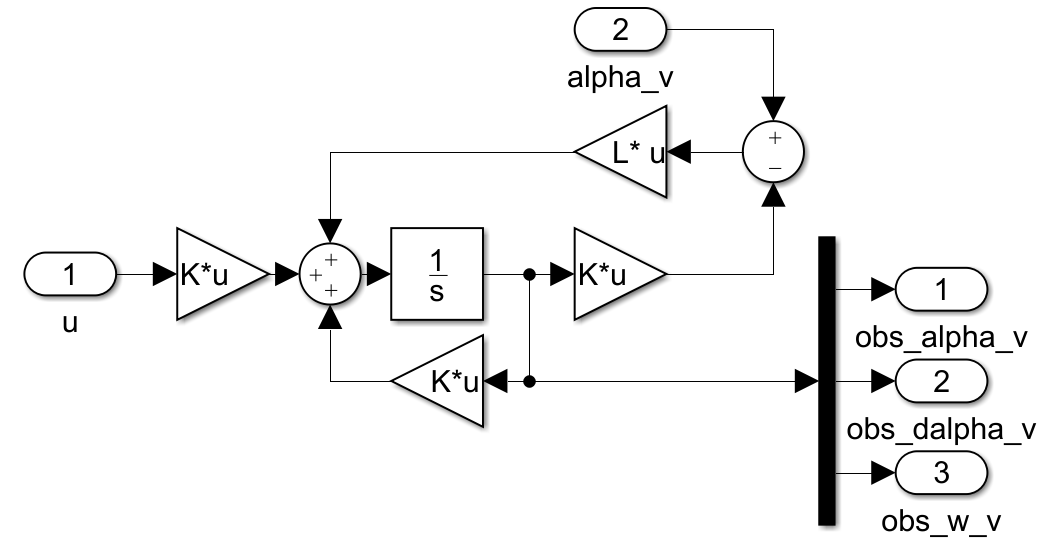
\includegraphics[width=4in]{Figures/Luenberger.png}
	\caption{Schemat blokowy realizujący obserwator Luenbergera.}
	\label{fig:Luenberger}
\end{figure}

Sprawdzono działanie obserwatora na zaimplementowanym modelu obiektu oraz na rzeczywistym obiekcie. Wykresy od \ref{fig:obsv_model_alpha_v} do \ref{fig:obsv_model_w_v} przedstawiają porównanie wyjścia obserwatora ze stanem modelowanego obiektu. Natomiast wykresy od \ref{fig:obsv_obj_alpha_v} do \ref{fig:obsv_obj_w_v} pokazują działanie obserwatora na rzeczywistym obiekcie.

\begin{figure}[H]
	\centering
	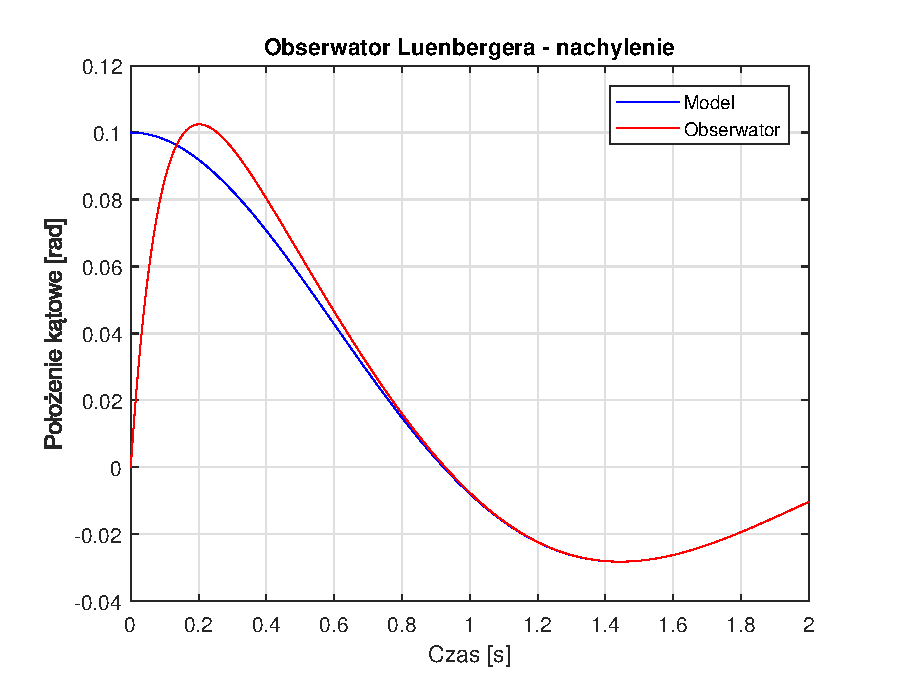
\includegraphics[width=4in]{Figures/obsv_model_alpha_v.eps}
	\caption{Porównanie nachylenia modelu z nachyleniem obserwatora.}
	\label{fig:obsv_model_alpha_v}
\end{figure}

\begin{figure}[H]
	\centering
	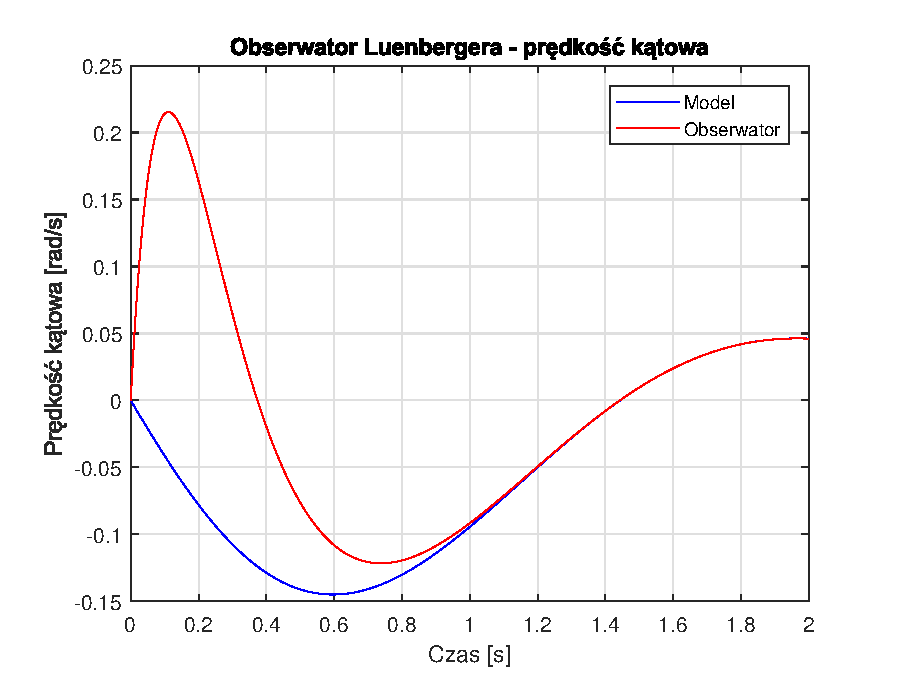
\includegraphics[width=4in]{Figures/obsv_model_dalpha_v.eps}
	\caption{Porównanie prędkości kątowej modelu z prędkością kątową obserwatora.}
	\label{fig:obsv_model_dalpha_v}
\end{figure}

\begin{figure}[H]
	\centering
	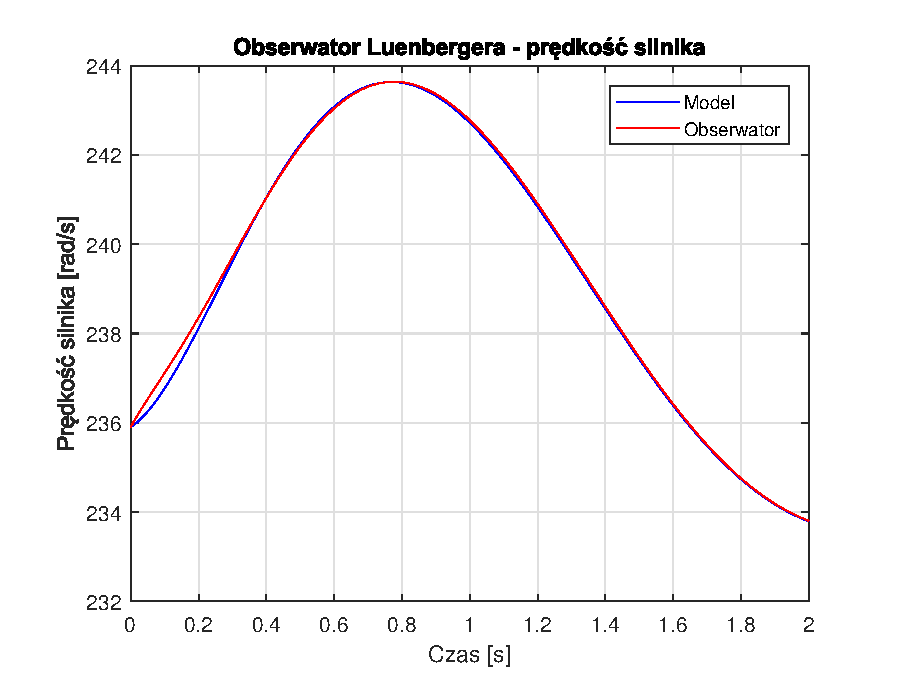
\includegraphics[width=4in]{Figures/obsv_model_w_v.eps}
	\caption{Porównanie prędkości silnika modelu z prędkością silnika obserwatora.}
	\label{fig:obsv_model_w_v}
\end{figure}

\begin{figure}[H]
	\centering
	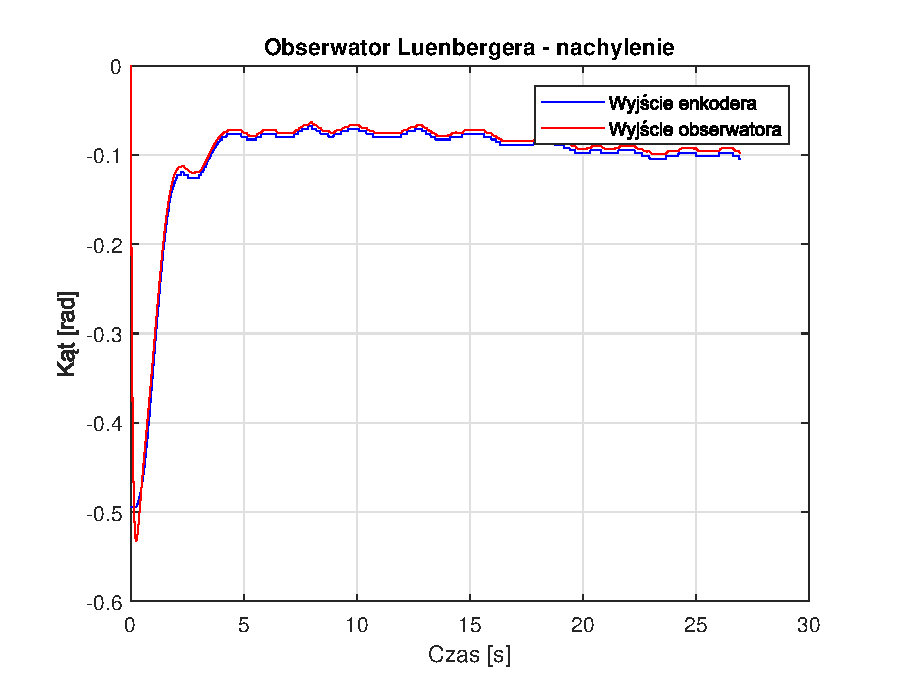
\includegraphics[width=4in]{Figures/obsv_obj_alpha_v.eps}
	\caption{Porównanie nachylenia obiektu z nachyleniem obserwatora.}
	\label{fig:obsv_obj_alpha_v}
\end{figure}

\begin{figure}[H]
	\centering
	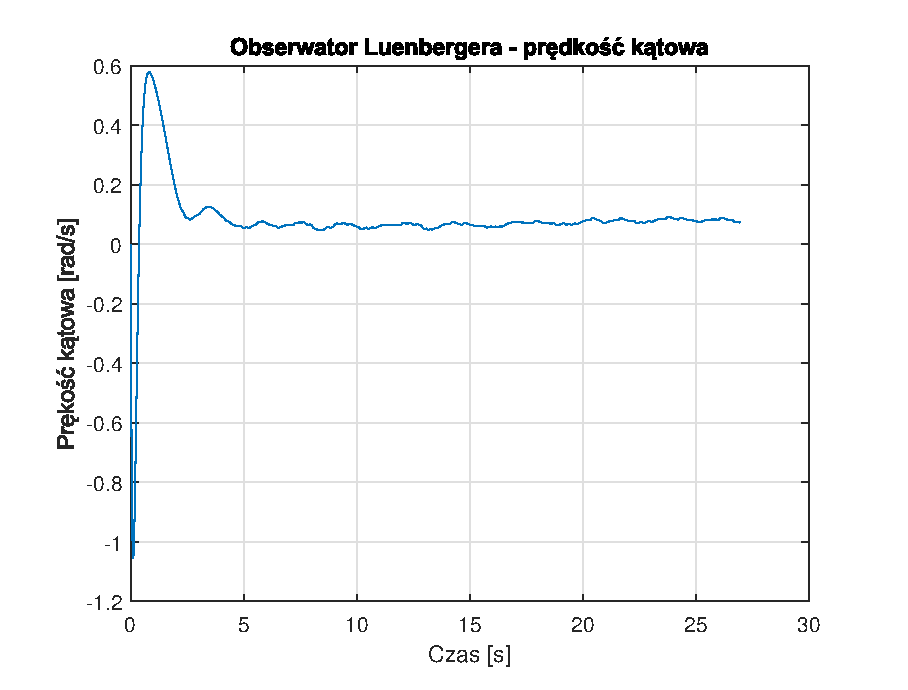
\includegraphics[width=4in]{Figures/obsv_obj_dalpha_v.eps}
	\caption{Prędkość kątowa obserwatora dla rzeczywistego obiektu.}
	\label{fig:obsv_obj_dalpha_v}
\end{figure}

\begin{figure}[H]
	\centering
	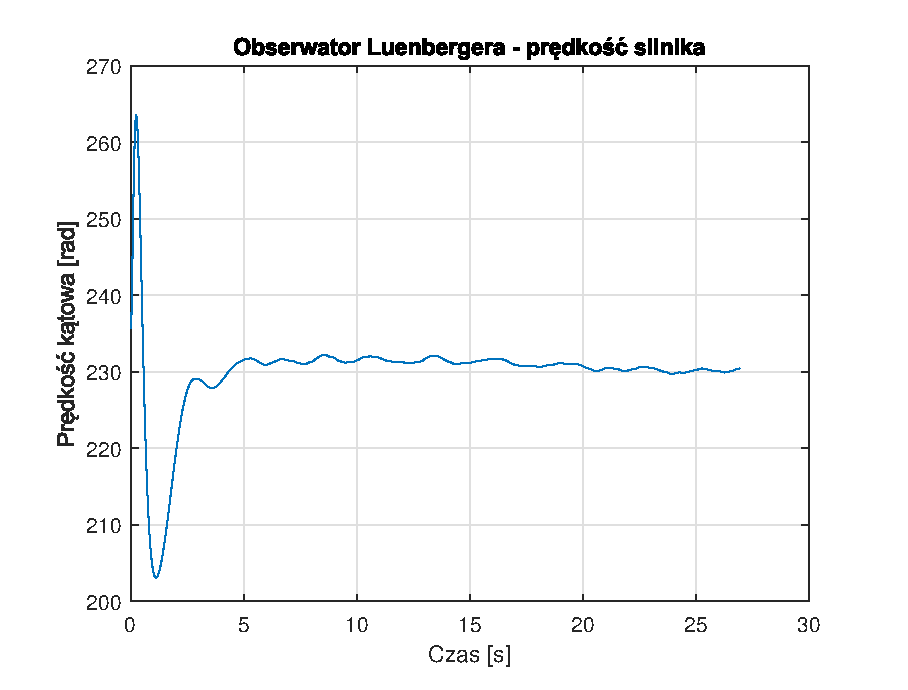
\includegraphics[width=4in]{Figures/obsv_obj_w_v.eps}
	\caption{Prędkość silnika obserwatora dla rzeczywistego obiektu.}
	\label{fig:obsv_obj_w_v}
\end{figure}

\section{Regulator LQ}
\label{sec:regulatorlq}
Dla układu zlinearyzowanego opisanego macierzami \eqref{eq:linear_ABCD_val} obliczono macierz wzmocnień regulatora LQ. Regulator ten minimalizuje następujący wskaźnik jakości:
\begin{equation}
\begin{aligned}
J&=\int\limits_0^{\infty}(x^TQx+u^TRu)dt\\
Q&=\begin{bmatrix}
1 & 0 & 0\\
0 & 0 & 0\\
0 & 0 & 0
\end{bmatrix}\\
R&=1
\end{aligned}
\end{equation}
Postać macierzy Q wskazuje, że celem jest jak najszybsza stabilizacja nachylenia układu, bez względu na pozostałe zmienne stanu. Potrzebne obliczenia (rozwiązanie algebraicznego równania Riccatiego) zostały wykonane za pomocą funkcji programu \textit{MATLAB} - \textit{lqr}. Otrzymana macierz wzmocnień ma następującą postać:
\begin{equation}
K=\begin{bmatrix}
-0.0861 & 0.4516 & 0.0030
\end{bmatrix}
\end{equation}
Regulator ten został następnie zaimplementowany w programie \textit{Simulink}. Układ z tym regulatorem został przedstawiony na rysunku \ref{fig:helikopter_lq}.

\begin{figure}[H]
	\centering
	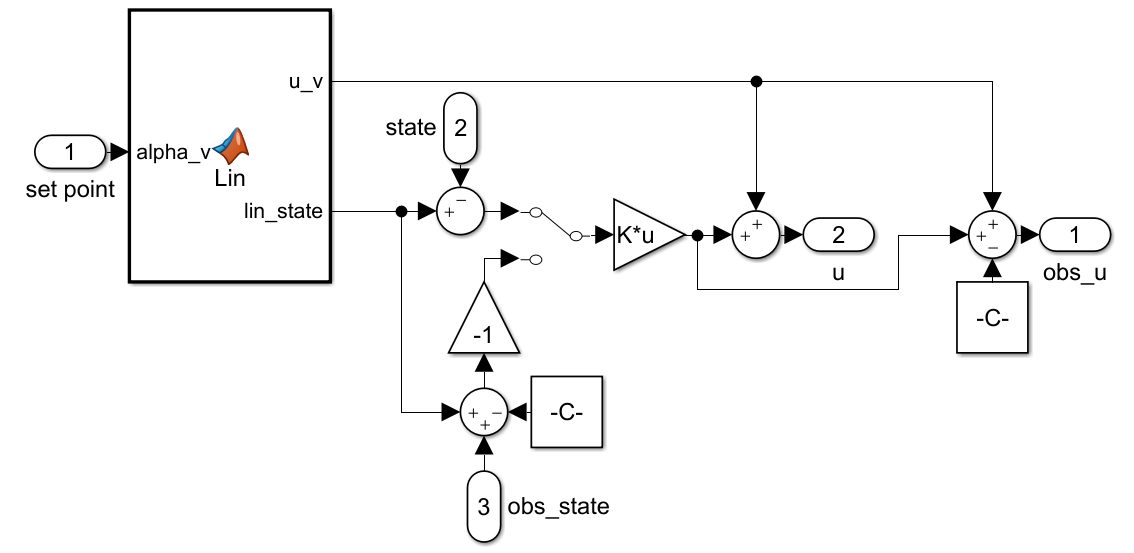
\includegraphics[width=5.9in]{Figures/helikopter_lq.png}
	\caption{Sterowanie układem z regulatorem LQ.}
	\label{fig:helikopter_lq}
\end{figure}

Użyty blok \textit{MATLAB function} służy do wyliczenia wartości zmiennych stanu oraz sterowania w zadanym punkcie równowagi. \textit{Manual switch} pozwala na zmianę działania układu między sterowaniem na podstawie wyjścia obserwatora Luenbergera lub na podstawie właściwych zmiennych stanu modelu. Na wykresach od \ref{fig:LQ_model_alpha_v} do \ref{fig:LQ_model_w_v} przedstawiono przebieg zmiennych stanu modelu z regulatorem LQ dla zadania stabilizacji, kiedy na wejście regulatora podawany był właściwy wektor stanu obiektu.

\begin{figure}[H]
	\centering
	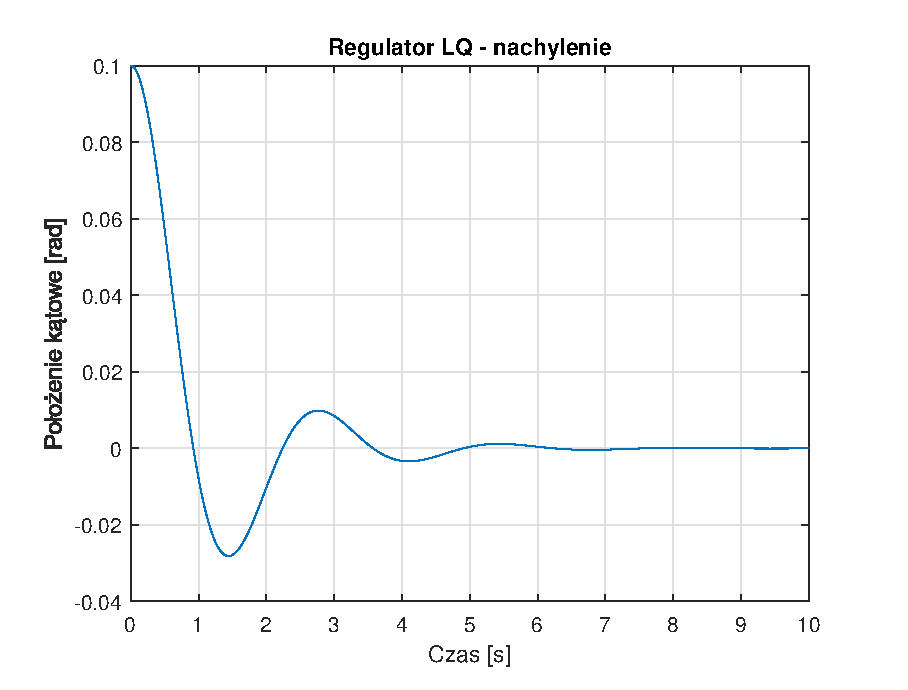
\includegraphics[width=4in]{Figures/LQ_model_alpha_v.eps}
	\caption{Przebieg nachylenia układu z regulatorem LQ.}
	\label{fig:LQ_model_alpha_v}
\end{figure}

\begin{figure}[H]
	\centering
	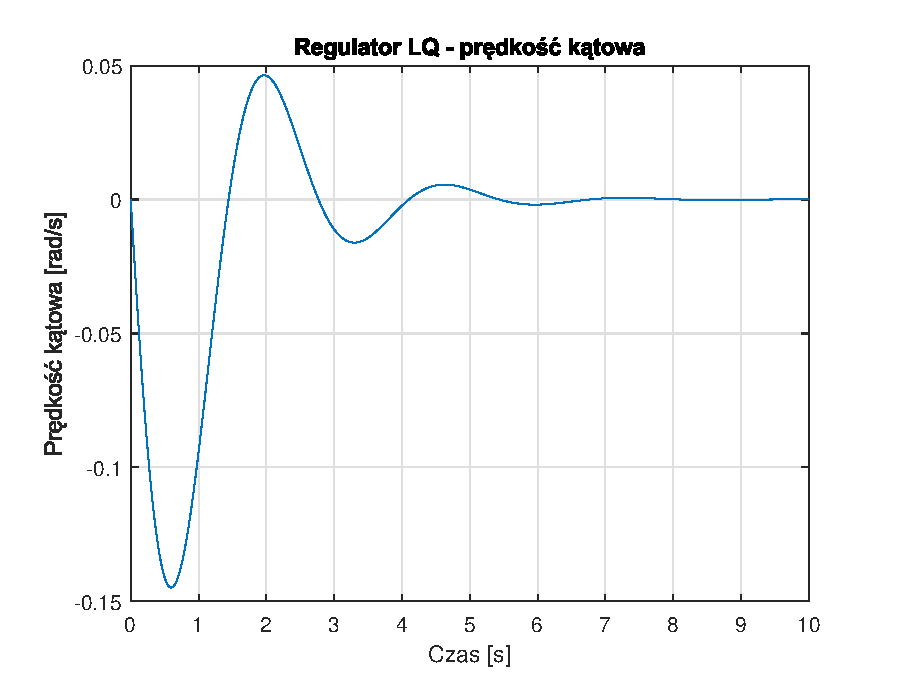
\includegraphics[width=4in]{Figures/LQ_model_dalpha_v.eps}
	\caption{Przebieg prędkości kątowej układu z regulatorem LQ.}
	\label{fig:LQ_model_dalpha_v}
\end{figure}

\begin{figure}[H]
	\centering
	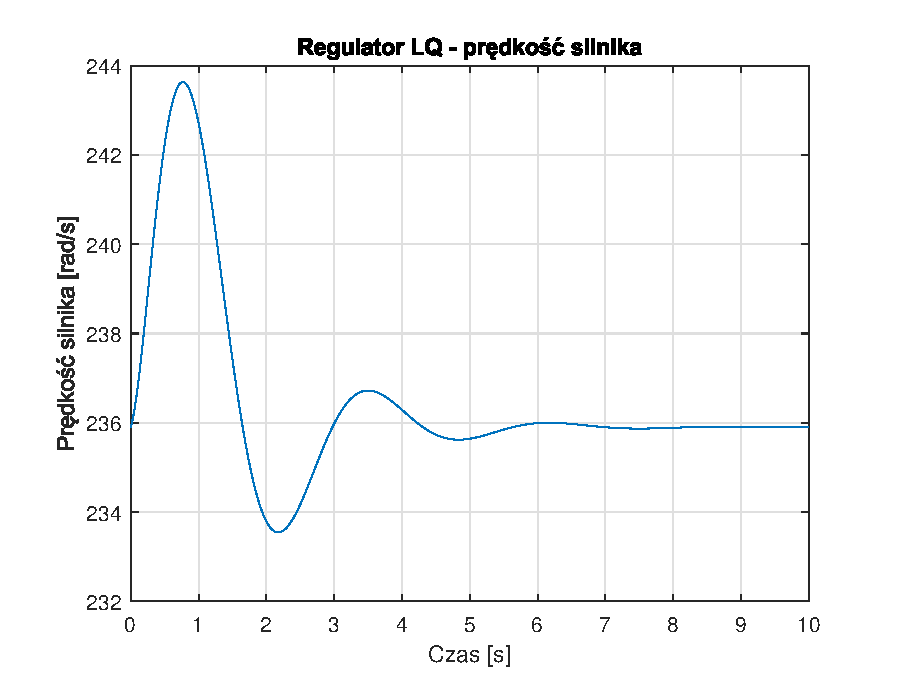
\includegraphics[width=4in]{Figures/LQ_model_w_v.eps}
	\caption{Przebieg prędkości silnika układu z regulatorem LQ.}
	\label{fig:LQ_model_w_v}
\end{figure}

Na wykresach od \ref{fig:LQ_model_03_alpha_v} do \ref{fig:LQ_model_03_w_v} przedstawiono przebieg zmiennych stanu modelu z regulatorem LQ dla zadania stabilizacji, kiedy na wejście regulatora podawany był właściwy wektor stanu obiektu. W tym wypadku jednak wartość zadana nie była punktem linearyzacji układu i wynosiła 0.3.

\begin{figure}[H]
	\centering
	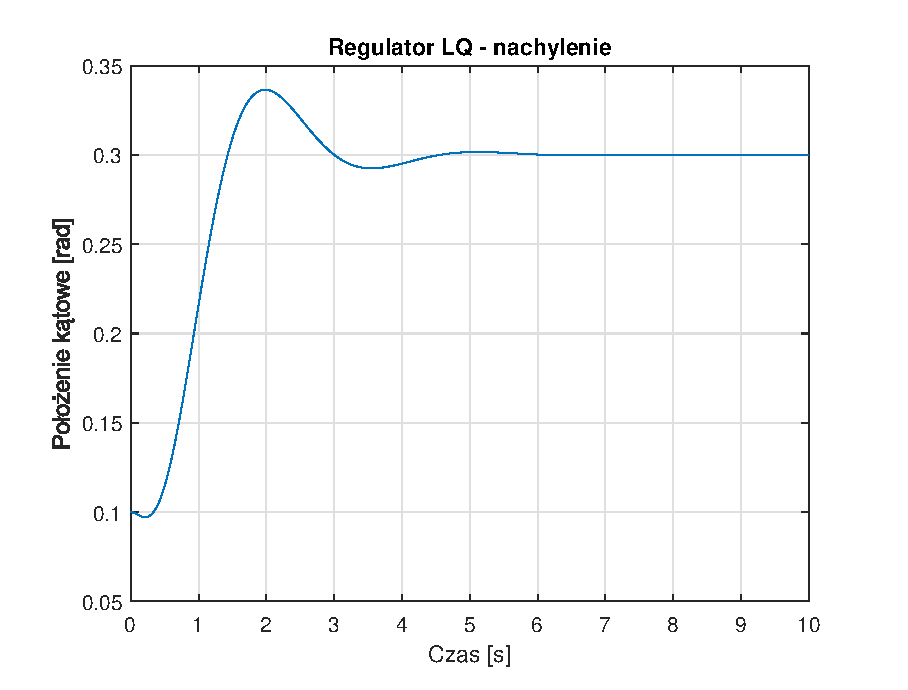
\includegraphics[width=4in]{Figures/LQ_model_03_alpha_v.eps}
	\caption{Przebieg nachylenia układu z regulatorem LQ.}
	\label{fig:LQ_model_03_alpha_v}
\end{figure}

\begin{figure}[H]
	\centering
	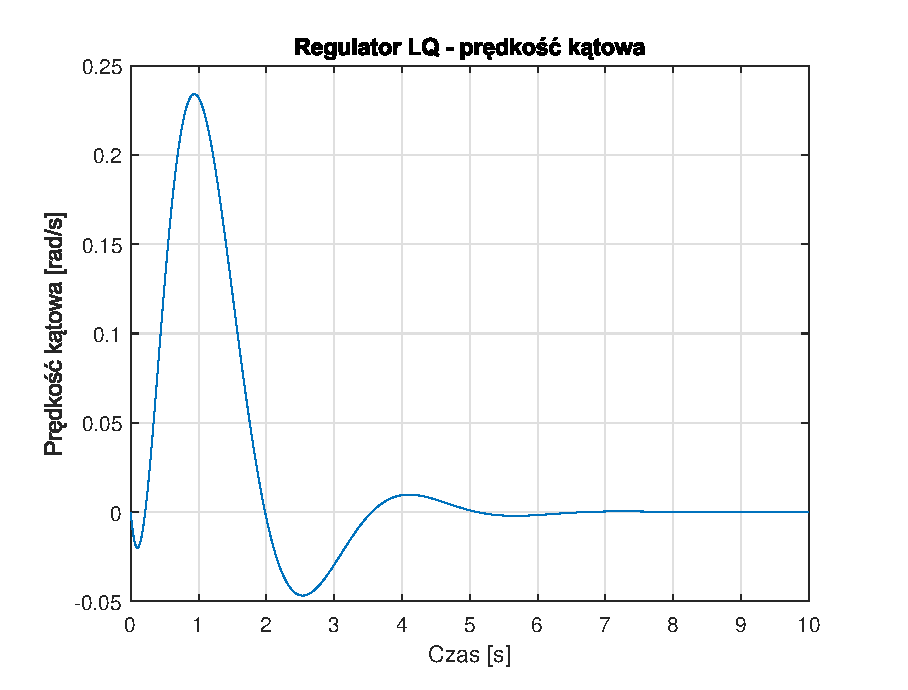
\includegraphics[width=4in]{Figures/LQ_model_03_dalpha_v.eps}
	\caption{Przebieg prędkości kątowej układu z regulatorem LQ.}
	\label{fig:LQ_model_03_dalpha_v}
\end{figure}

\begin{figure}[H]
	\centering
	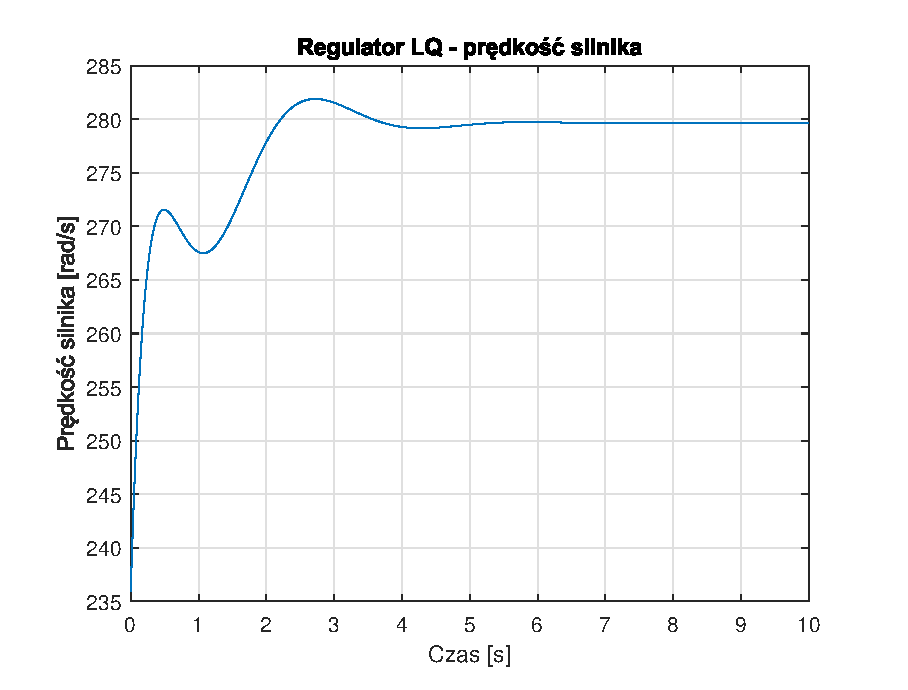
\includegraphics[width=4in]{Figures/LQ_model_03_w_v.eps}
	\caption{Przebieg prędkości silnika układu z regulatorem LQ.}
	\label{fig:LQ_model_03_w_v}
\end{figure}

Na wykresach od \ref{fig:LQ_model_obs_03_alpha_v} do \ref{fig:LQ_model_obs_03_w_v} przedstawiono przebieg zmiennych stanu modelu z regulatorem LQ dla zadania stabilizacji, kiedy na wejście regulatora podawany był wektor stanu obiektu obliczony z pomocą obserwatora Luenbergera. Wartość zadana nie była punktem linearyzacji układu i wynosiła 0.3.

\begin{figure}[H]
	\centering
	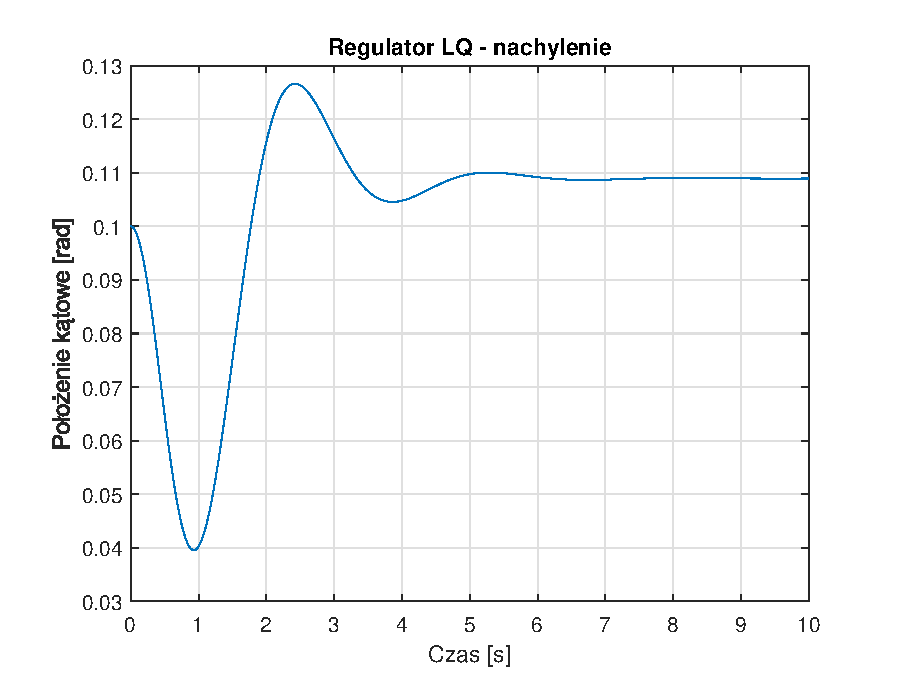
\includegraphics[width=4in]{Figures/LQ_model_obs_03_alpha_v.eps}
	\caption{Przebieg nachylenia układu z regulatorem LQ.}
	\label{fig:LQ_model_obs_03_alpha_v}
\end{figure}

\begin{figure}[H]
	\centering
	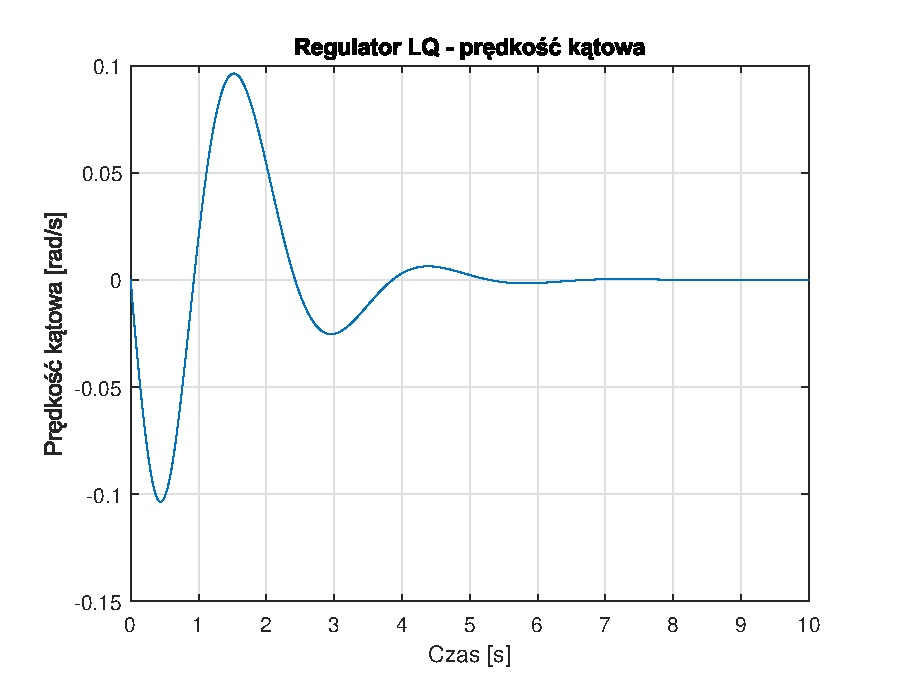
\includegraphics[width=4in]{Figures/LQ_model_obs_03_dalpha_v.eps}
	\caption{Przebieg prędkości kątowej układu z regulatorem LQ.}
	\label{fig:LQ_model_obs_03_dalpha_v}
\end{figure}

\begin{figure}[H]
	\centering
	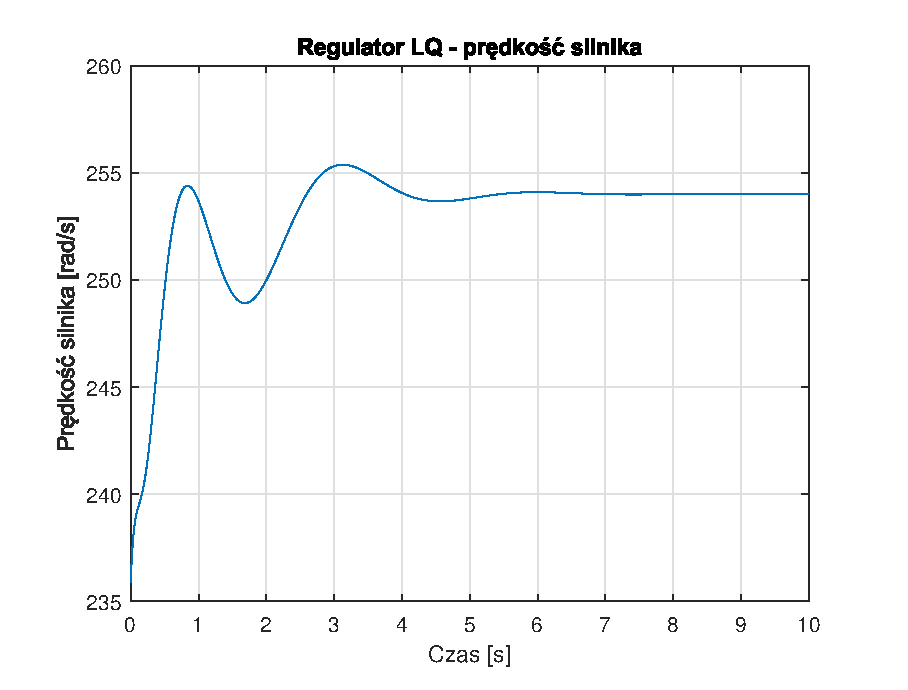
\includegraphics[width=4in]{Figures/LQ_model_obs_03_w_v.eps}
	\caption{Przebieg prędkości silnika układu z regulatorem LQ.}
	\label{fig:LQ_model_obs_03_w_v}
\end{figure}

W tym wypadku widoczny jest wyraźny uchyb ustalony.

\section{Regulator LQI}
\label{sec:regulatorlqi}
Dla układu zlinearyzowanego opisanego macierzami \eqref{eq:linear_ABCD_val} obliczono macierz wzmocnień regulatora LQI. Regulator ten minimalizuje następujący wskaźnik jakości:
\begin{equation}
\begin{aligned}
J&=\int\limits_0^{\infty}(x^TQx+u^TRu)dt\\
Q&=\begin{bmatrix}
1 & 0 & 0 & 0\\
0 & 0 & 0 & 0\\
0 & 0 & 0 & 0\\
0 & 0 & 0 & 1
\end{bmatrix}\\
R&=1
\end{aligned}
\end{equation}
\noindent gdzie:\newline
\(x_4\) jest całką z uchybu kąta.
\paragraph*{}
Postać macierzy Q wskazuje, że celem jest jak najszybsza stabilizacja nachylenia układu oraz eliminacja uchybu ustalonego, bez względu na pozostałe zmienne stanu. Potrzebne obliczenia (rozwiązanie algebraicznego równania Riccatiego) zostały wykonane za pomocą funkcji programu \textit{MATLAB} - \textit{lqi}. Otrzymana macierz wzmocnień ma następującą postać:
\begin{equation}
K=\begin{bmatrix}
0.3154 & 0.7105 & 0.0042 & -1
\end{bmatrix}
\end{equation}
Regulator ten został następnie zaimplementowany w programie \textit{Simulink}. Układ z tym regulatorem został przedstawiony na rysunku \ref{fig:helikopter_lq}.

\begin{figure}[H]
	\centering
	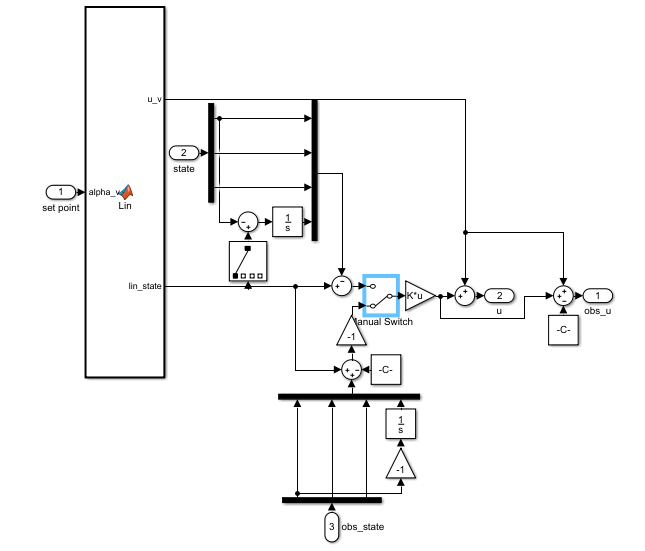
\includegraphics[width=5.9in]{Figures/helikopter_lqi.png}
	\caption{Sterowanie układem z regulatorem LQI.}
	\label{fig:helikopter_lqi}
\end{figure}

Użyty blok \textit{MATLAB function} służy do wyliczenia wartości zmiennych stanu oraz sterowania w zadanym punkcie równowagi. \textit{Manual switch} pozwala na zmianę działania układu między sterowaniem na podstawie wyjścia obserwatora Luenbergera lub na podstawie właściwych zmiennych stanu modelu. Można zauważyć również całkę odpowiedzialnych za wprowadzoną, sztuczną zmienną stanu. Na wykresach od \ref{fig:LQI_model_alpha_v} do \ref{fig:LQI_model_w_v} przedstawiono przebieg zmiennych stanu modelu z regulatorem LQI dla zadania stabilizacji, kiedy na wejście regulatora podawany był właściwy wektor stanu obiektu.

\begin{figure}[H]
	\centering
	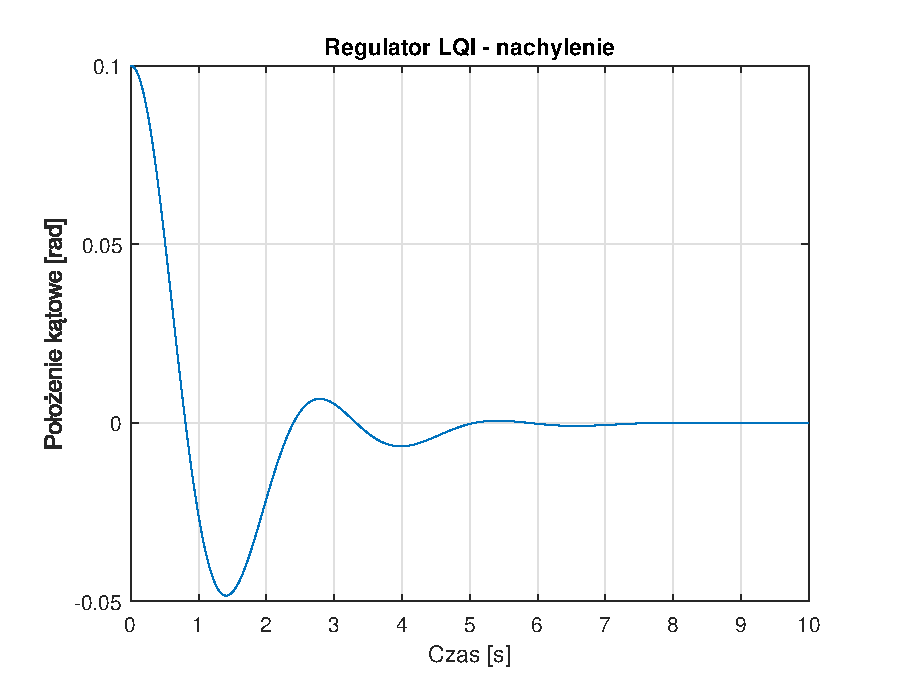
\includegraphics[width=4in]{Figures/LQI_model_alpha_v.eps}
	\caption{Przebieg nachylenia układu z regulatorem LQI.}
	\label{fig:LQI_model_alpha_v}
\end{figure}

\begin{figure}[H]
	\centering
	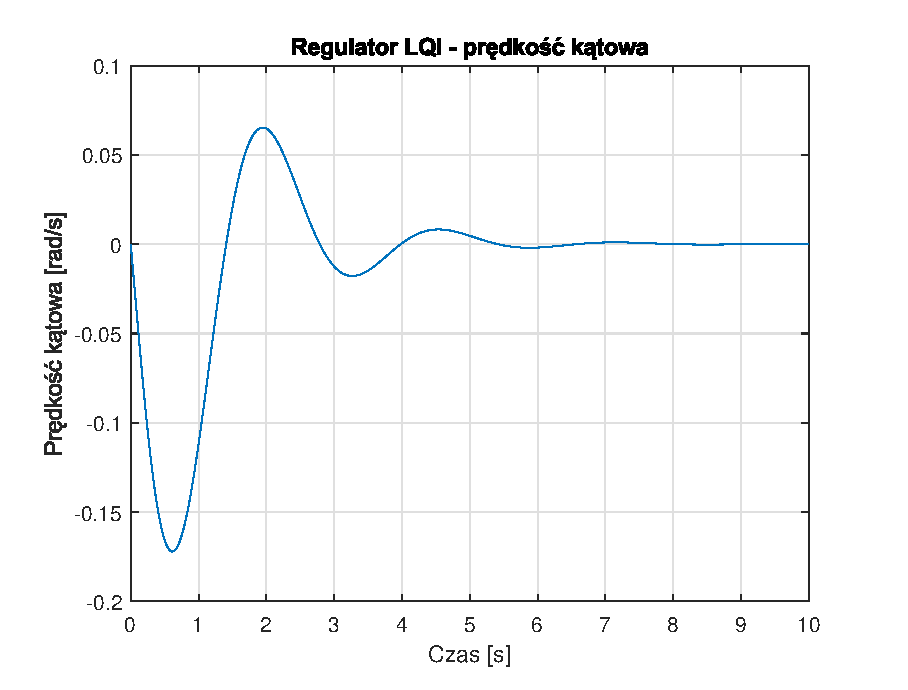
\includegraphics[width=4in]{Figures/LQI_model_dalpha_v.eps}
	\caption{Przebieg prędkości kątowej układu z regulatorem LQI.}
	\label{fig:LQI_model_dalpha_v}
\end{figure}

\begin{figure}[H]
	\centering
	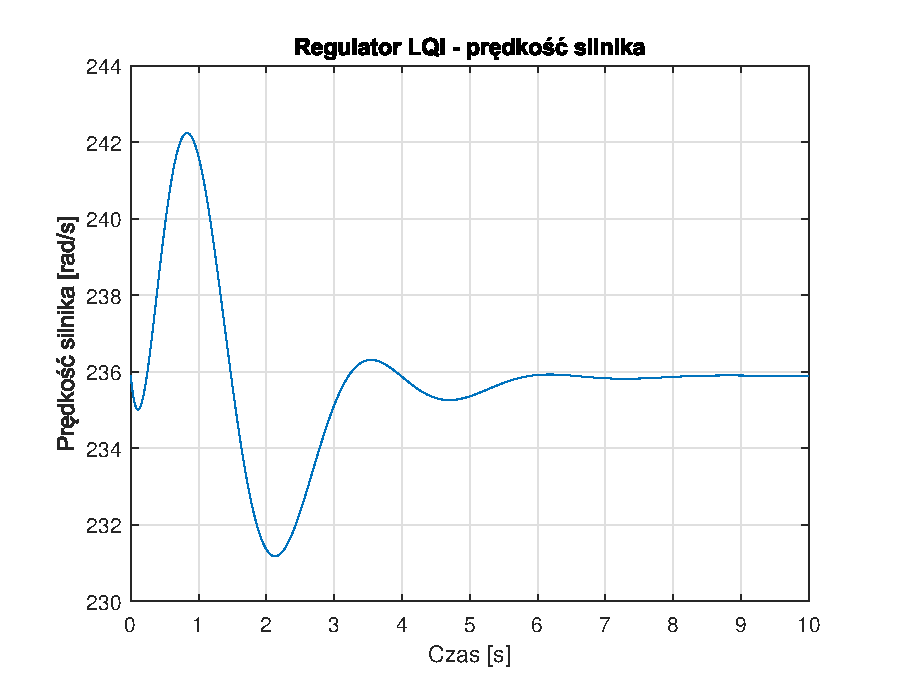
\includegraphics[width=4in]{Figures/LQI_model_w_v.eps}
	\caption{Przebieg prędkości silnika układu z regulatorem LQI.}
	\label{fig:LQI_model_w_v}
\end{figure}

Na wykresach od \ref{fig:LQI_model_03_alpha_v} do \ref{fig:LQI_model_03_w_v} przedstawiono przebieg zmiennych stanu modelu z regulatorem LQI dla zadania stabilizacji, kiedy na wejście regulatora podawany był właściwy wektor stanu obiektu. W tym wypadku jednak wartość zadana nie była punktem linearyzacji układu i wynosiła 0.3.

\begin{figure}[H]
	\centering
	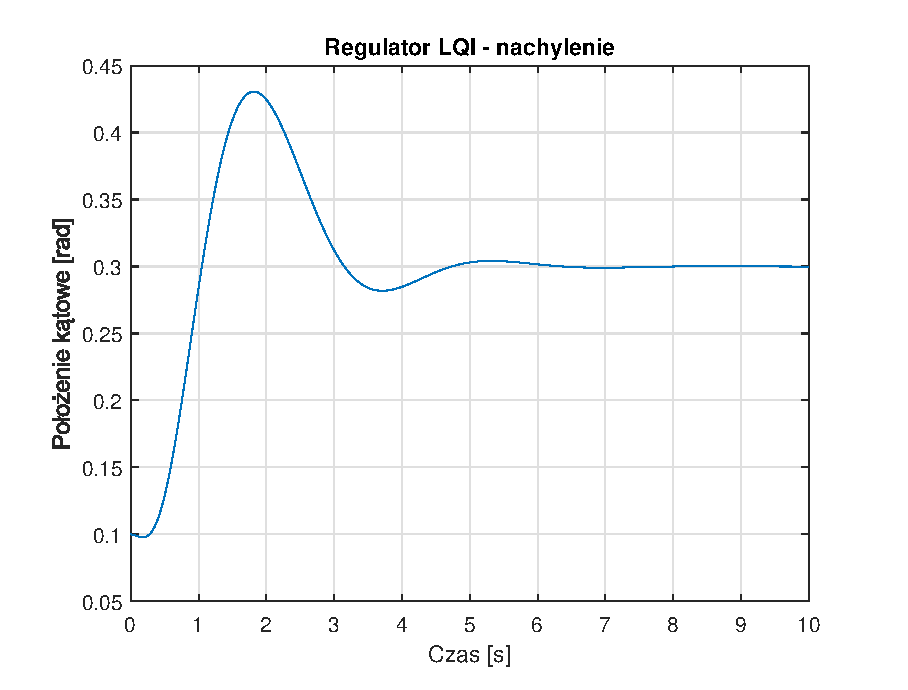
\includegraphics[width=4in]{Figures/LQI_model_03_alpha_v.eps}
	\caption{Przebieg nachylenia układu z regulatorem LQI.}
	\label{fig:LQI_model_03_alpha_v}
\end{figure}

\begin{figure}[H]
	\centering
	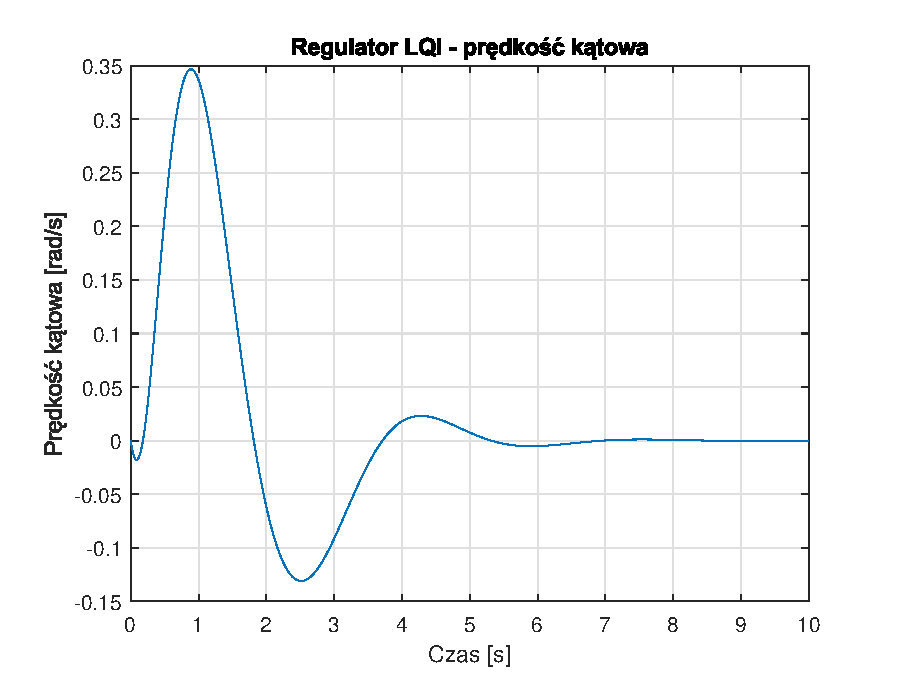
\includegraphics[width=4in]{Figures/LQI_model_03_dalpha_v.eps}
	\caption{Przebieg prędkości kątowej układu z regulatorem LQI.}
	\label{fig:LQI_model_03_dalpha_v}
\end{figure}

\begin{figure}[H]
	\centering
	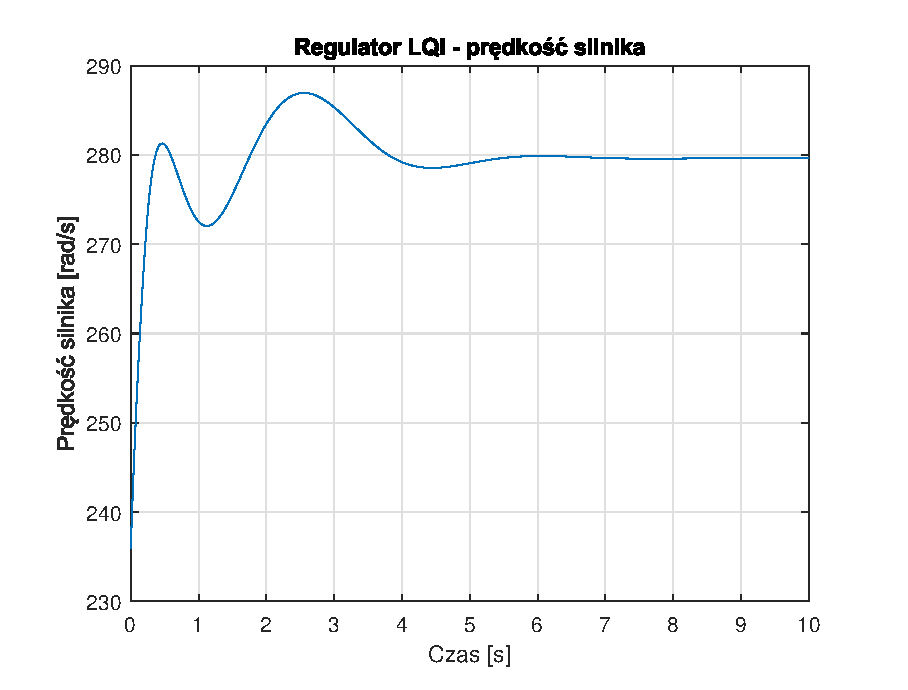
\includegraphics[width=4in]{Figures/LQI_model_03_w_v.eps}
	\caption{Przebieg prędkości silnika układu z regulatorem LQI.}
	\label{fig:LQI_model_03_w_v}
\end{figure}

Na wykresach od \ref{fig:LQI_model_obs_03_alpha_v} do \ref{fig:LQI_model_obs_03_w_v} przedstawiono przebieg zmiennych stanu modelu z regulatorem LQI dla zadania stabilizacji, kiedy na wejście regulatora podawany był wektor stanu obiektu obliczony z pomocą obserwatora Luenbergera. Wartość zadana nie była punktem linearyzacji układu i wynosiła 0.3.

\begin{figure}[H]
	\centering
	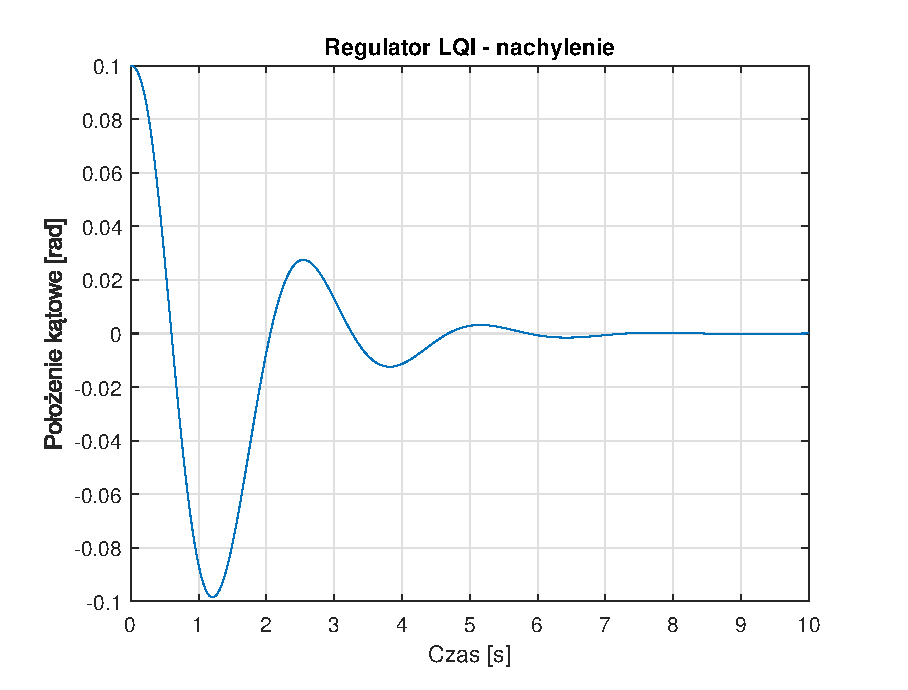
\includegraphics[width=4in]{Figures/LQI_model_obs_03_alpha_v.eps}
	\caption{Przebieg nachylenia układu z regulatorem LQI.}
	\label{fig:LQI_model_obs_03_alpha_v}
\end{figure}

\begin{figure}[H]
	\centering
	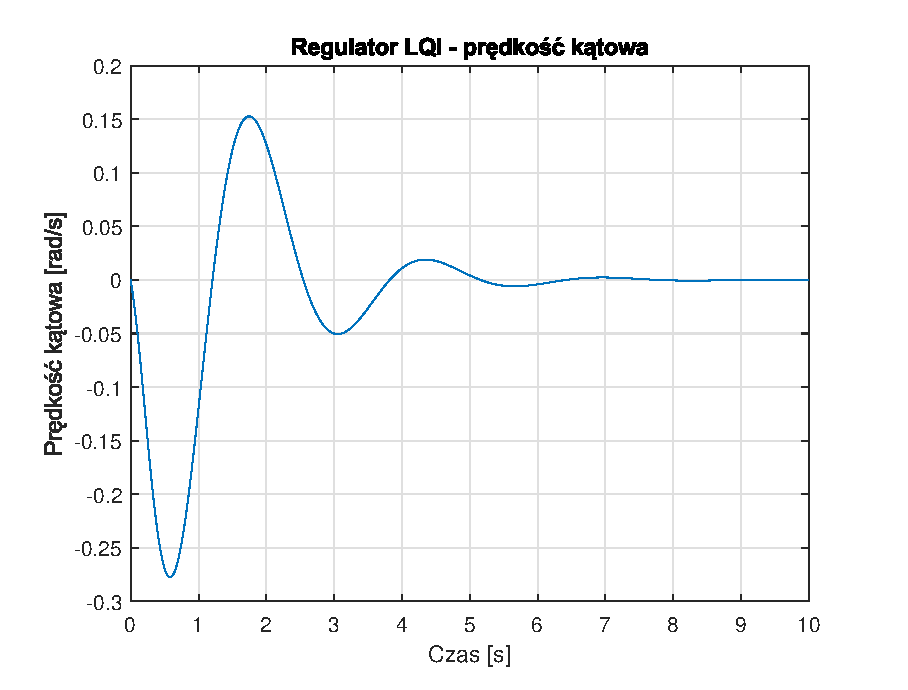
\includegraphics[width=4in]{Figures/LQI_model_obs_03_dalpha_v.eps}
	\caption{Przebieg prędkości kątowej układu z regulatorem LQI.}
	\label{fig:LQI_model_obs_03_dalpha_v}
\end{figure}

\begin{figure}[H]
	\centering
	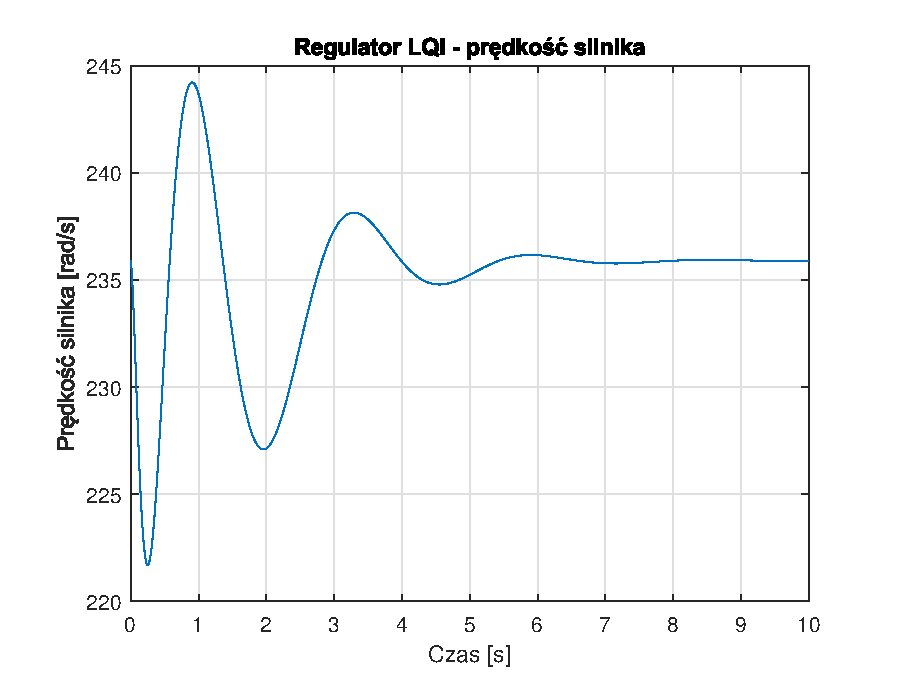
\includegraphics[width=4in]{Figures/LQI_model_obs_03_w_v.eps}
	\caption{Przebieg prędkości silnika układu z regulatorem LQI.}
	\label{fig:LQI_model_obs_03_w_v}
\end{figure}

Używając regulatora LQI udało się więc wyeliminować uchyb ustalony, który występował dla regulatora LQ.

\section{Regulator PID}
Postanowiono również sprawdzić jak klasyczny regulator PID poradzi sobie z zadaniem regulacji dla danego obiektu. W tym celu, na drodze doświadczalnej zaprojektowano układ regulacji składający się z dwóch regulatorów PID. Pierwszy z nich był odpowiedzialny za doprowadzenie obiektu w pobliże wartości zadanej tzn. \(\pm\ang{10}\), tłumiąc jednocześnie występujące w układzie oscylacje. Drugi natomiast zapewniał pozycjonowanie helikoptera w zadanym położeniu. Schemat omawianego układu zaprezentowany jest na rysunku \ref{fig:pid_schemat}, natomiast wartości nastaw poszczególnych parametrów znajdują się w tabeli \ref{nastawy_pid} 
%Ze względu na charakterystyki obu regulatorów pierwszy miał małe wzmocnienie części całkującej i duże części różniczkującej,   

\begin{figure}[H]
	\centering
	\includegraphics[width=5.9in]{Figures/PID_schemat.png}
	\caption{Schemat układu sterowania dla regulatorów PID.}
	\label{fig:pid_schemat}
\end{figure}

\begin{table}[ht]
	\caption{Wartości nastaw regulatorów PID.}
	\label{nastawy_pid}
	\centering
	
	\begin{tabular}{|c|c|c|c|}
		\hline
		Regulator &P&I&D\\
		\hline
		Reg. nr 1 &0.025&   0 &  0.035\\
		\hline
		Reg. nr 2 &0.2 &0.012 &0.015\\ 
		\hline
	\end{tabular}
\end{table}

Ze względu na to, że zadaniem pierwszego regulatora było jak najszybsze doprowadzenie obiektu w okolice wartości zadanej i wyeliminowanie oscylacji, to wartość wzmocnienia części różniczkującej jest większa niż w przypadku drugiego regulatora. Analogiczna zależność zachodzi dla regulatora nr 2 i części całkującej, której to wartości jest większa niż w pierwszym przypadku. \\
Głównym problemem w projektowaniu tego układu było odpowiednie ograniczenie członu całkującego regulatora nr 2, w momencie gdy ten nie był aktywny. Na drodze przeprowadzonych eksperymentów  ustalono, że najlepiej będzie podawać na ten regulator 0.1 wartości uchybu w sytuacji, gdy jest on nieaktywny. Dzięki temu człon całkujący nie osiągał aż tak dużej wartości, która wprowadziłaby do układu oscylacje, i jednocześnie generował na tyle duże sterowanie, że układ był sprowadzany do zadanej pozycji od momentu aktywacji regulatora.  Na rysunku \ref{fig:PID_30} zaprezentowano działanie całego układu.

\begin{figure}[H]
	\centering
	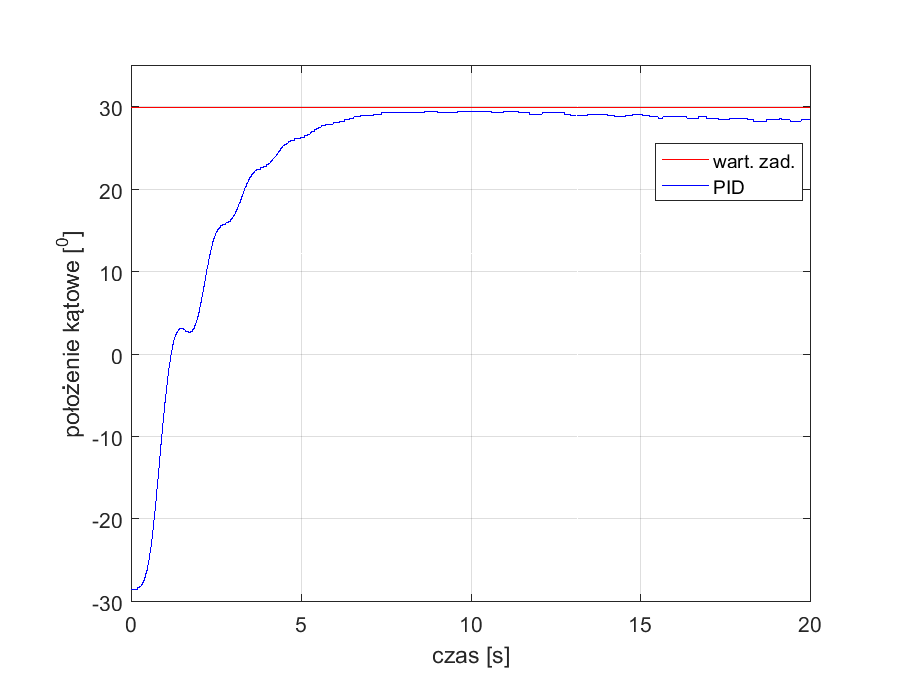
\includegraphics[width=4in]{Figures/pid30.eps}
	\caption{Działanie regulatora PID dla stabilizacji w położeniu \ang{30}.}
	\label{fig:PID_30}
\end{figure}

\newpage
\section{Porównanie działania regulatorów}

Działanie zaprojektowanych regulatorów zostało sprawdzone w następujących przypadkach: 
\begin{enumerate}
	\item działanie regulatorów LQ i LQI z i bez obserwatora,
	\item pozycjonowanie w pozycji \ang{0},
	\item pozycjonowanie w pozycji \ang{10},
	\item pozycjonowanie w pozycji \ang{20},
	\item stabilizacja układu dla regulatora LQ i sterowania początkowego wyliczonego w innym punkcie niż wartość zadana,
	\item zadanie nadążania.
\end{enumerate}
Aby móc porównać jakość sterowania w każdym z wymienionych powyżej przypadków zdefiniowano całkowy wskaźnik jakość:
\begin{equation}\label{key}
J =\int_{0}^{T} e^2(t) dt
\end{equation}

\subsection{Porównanie działania regulatorów LQ i LQI z i bez obserwatora}
W tym przypadku sprawdzono jak włączenie do układu regulacji obserwatora wpłynęło na jakość regulacji. Jak można zauważyć na rys. \ref{fig:por_LQ0} i \ref{fig:por_LQ0obs} po zastosowaniu obserwatora przeregulowanie dla regulatora LQI zmalało z $23.28 ^0$ do $ 20.92$, natomiast dla regulatora LQ widać znaczącą redukcję oscylacji. Wartości wskaźnika jakości dla wszystkich czterech przypadków znajdują się w tabeli \ref{obs_por_tab}.

\begin{table}[ht]
	\caption{Wskaźniki jakości dla układu z i bez obserwatora.}
	\label{obs_por_tab}
	\centering
	
	\begin{tabular}{|c|c|}
		\hline
		przypadek &J\\
		\hline
		Reg. LQ & $5.2031\cdot 10 ^3$\\
		\hline
		Reg. LQ + obserwator & $5.7391 \cdot 10 ^3$\\
		\hline
		Reg. LQI & $2.9717 \cdot 10 ^3$\\
		\hline
		Reg. LQI + obserwator & $2.9310 \cdot 10 ^3$\\ 
		\hline
	\end{tabular}
\end{table}

\begin{figure}[H]
	\centering
	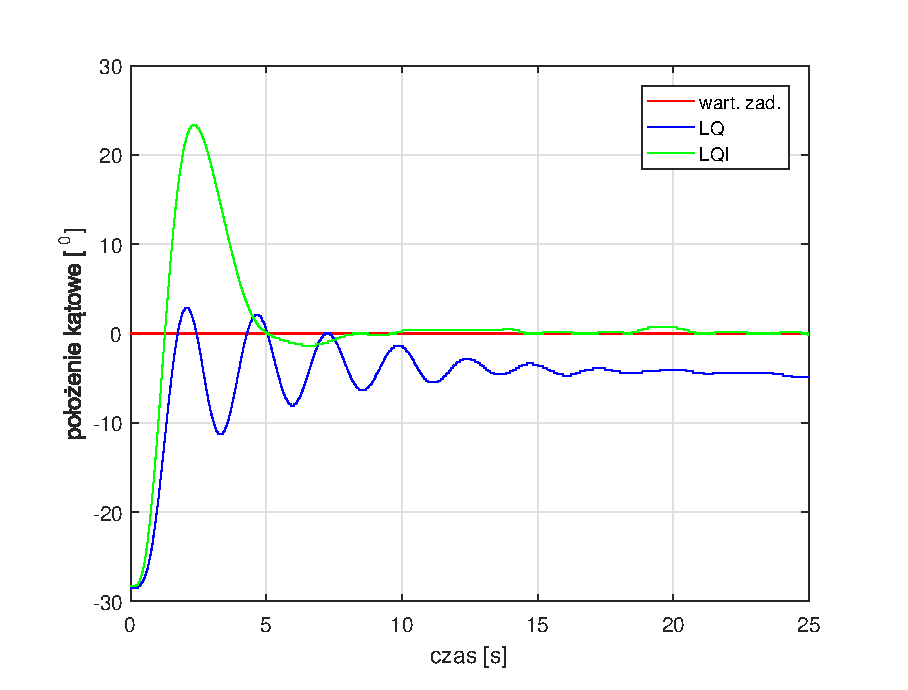
\includegraphics[width=4in]{Figures/por_LQ0.eps}
	\caption{Porównanie działania regulatorów LQI i LQ dla stabilizacji w położeniu \ang{0} bez obserwatora.}
	\label{fig:por_LQ0}
\end{figure}

\begin{figure}[H]
	\centering
	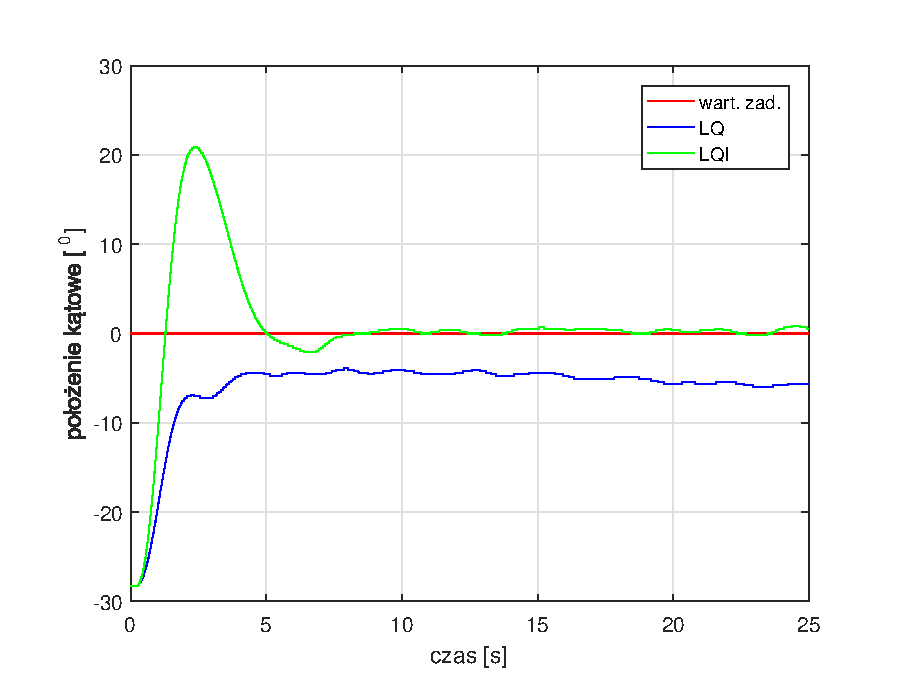
\includegraphics[width=4in]{Figures/por_LQ0obs.eps}
	\caption{Porównanie działania regulatorów LQI i LQ dla stabilizacji w położeniu \ang{0} z obserwatorem.}
	\label{fig:por_LQ0obs}
\end{figure}

\subsection{Stabilizacja w położeniu \texorpdfstring{\ang{0}}{Lg}}
W przypadku stabilizacji w położeniu \ang{0} porównano ze sobą wszystkie trzy typy regulatorów. Wartości wskaźnika jakości dla każdego z przypadków zamieszczone są w tabeli \ref{por_reg_0_tab}. Jak można zauważyć na rys. \ref{fig:por_LQPID_0} najlepiej z zadaniem stabilizacji poradził sobie regulator PID. 

\begin{table}[ht]
	\caption{Wskaźniki jakości dla stabilizacji w położeniu \ang{0}.}
	\label{por_reg_0_tab}
	\centering
	
	\begin{tabular}{|c|c|}
		\hline
		Regulator &J\\
		\hline
		LQ & $1.2540 \cdot 10 ^3$\\
		\hline
		LQI & $1.2775 \cdot 10 ^3$\\
		\hline
		PID & $ 1.0293 \cdot 10 ^3$\\ 
		\hline
	\end{tabular}
\end{table}

\begin{figure}[H]
	\centering
	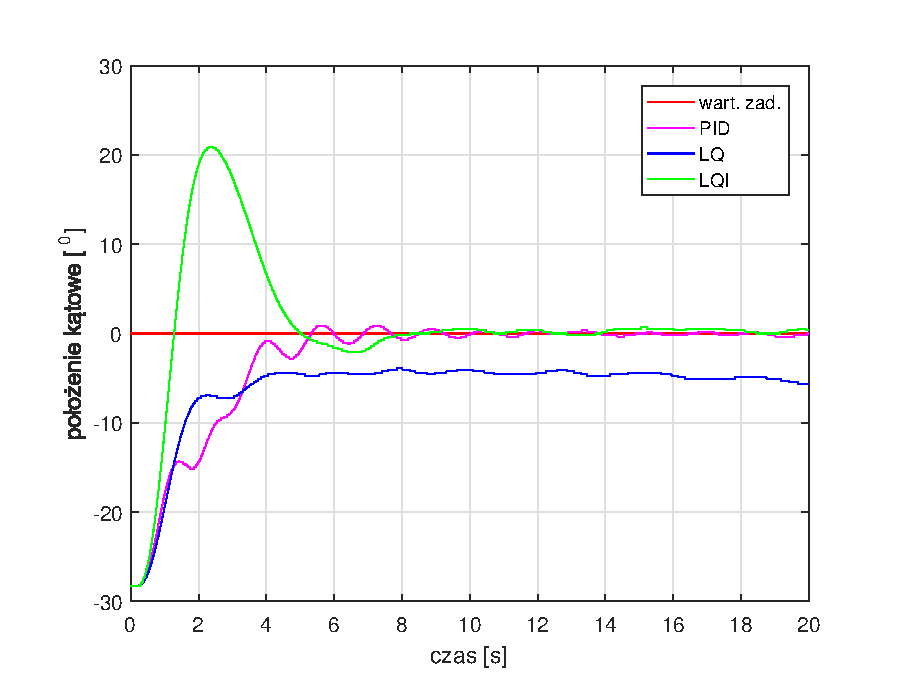
\includegraphics[width=4in]{Figures/por_LQ0PID.eps}
	\caption{Porównanie działania regulatora PID LQ i LQI dla stabilizacji w położeniu \ang{0}.}
	\label{fig:por_LQPID_0}
\end{figure}

\subsection{Stabilizacja w położeniu \texorpdfstring{\ang{10}}{Lg}}
Wartości wskaźnika jakości podane są w tabeli \ref{por_reg_10_tab}

\begin{table}[ht]
	\caption{Wskaźniki jakości dla stabilizacji w położeniu \ang{10}.}
	\label{por_reg_10_tab}
	\centering
	
	\begin{tabular}{|c|c|}
		\hline
		Regulator &J\\
		\hline
		LQ & $1.4181 \cdot 10 ^3$\\
		\hline
		LQI & $1.8473 \cdot 10 ^3$\\
		\hline
	\end{tabular}
\end{table}


\begin{figure}[H]
	\centering
	\includegraphics[width=4in]{Figures/por_LQ18.eps}
	\caption{Porównanie działania regulatorów LQI i LQ dla stabilizacji w położeniu \ang{10}.}
	\label{fig:por_LQ10}
\end{figure}

\subsection{Stabilizacja w położeniu \texorpdfstring{\ang{20}}{Lg}}

Wartości wskaźnika jakości podane są w tabeli \ref{por_reg_20_tab}

\begin{table}[ht]
	\caption{Wskaźniki jakości dla stabilizacji w położeniu \ang{20}.}
	\label{por_reg_20_tab}
	\centering
	
	\begin{tabular}{|c|c|}
		\hline
		Regulator &J\\
		\hline
		LQ & $2.6635 \cdot 10 ^3$\\
		\hline
		LQI & $2.9310 \cdot 10 ^3$\\
		\hline
	\end{tabular}
\end{table}

\begin{figure}[H]
	\centering
	\includegraphics[width=4in]{Figures/por_LQ9.eps}
	\caption{Porównanie działania regulatorów LQI i LQ dla stabilizacji w położeniu \ang{20}.}
	\label{fig:por_LQ20}
\end{figure}

\subsection{Stabilizacja dla sterowania wyliczonego w innym punkcie niż wartość zadana.}
Z tabeli \ref{por_reg_LQ_u0} i wykresu \ref{fig:por_LQ9_u} wynika, że zaniedbanie linearyzacji modelu rozważanego układu, w celu wyliczenia $u_0$ dla stabilizacji w różnych pozycjach, w znaczący sposób przekłada się na jakość sterowania. Odpowiednio wskaźnik jakości \textit{J} jak i również przeregulowanie i uchyb ustalony są gorsze dla regulatora zlinearyzowanego w położeniu \ang{0}. 
\begin{table}[ht]
	\caption{Wskaźniki jakości dla stabilizacji w położeniu \ang{20} dla różnych wartości $u_0$.}
	\label{por_reg_LQ_u0}
	\centering
	
	\begin{tabular}{|c|c|}
		\hline
		Punkt pracy &J\\
		\hline
		\ang{0} & $2.7635 \cdot 10 ^3$\\
		\hline
		\ang{20} & $2.7306 \cdot 10 ^3$\\
		\hline
	\end{tabular}
\end{table}

\begin{figure}[H]
	\centering
	\includegraphics[width=4in]{Figures/porLQ9_u.eps}
	\caption{Porównanie działania regulatora LQ dla stabilizacji w położeniu \ang{20} dla sterowania początkowego wyliczonego w punkcie \ang{0} i \ang{20}.}
	\label{fig:por_LQ9_u}
\end{figure}

%
%\begin{figure}[H]
%	\centering
%	\includegraphics[width=4in]{Figures/porLQ18_u.eps}
%	\caption{Porównanie działania regulatora LQ dla stabilizacji w położeniu $+10 ^0$ dla sterowania początkowego wyliczonego w punkcie $0^0$ i $10^0$.}
%	\label{fig:por_LQ18_u}
%\end{figure}

\subsection{Zadanie nadążania}
Na podstawie wykresu \ref{fig:por_foll_LQILQ} wynika, że regulator LQI poradził sobie zdecydowanie lepiej z zadaniem nadążania niż regulator LQ. Opóźnienie pomiędzy wartością zadaną, a pozycją helikoptera wynosi dla regulatora LQI $2.22 \ s$, natomiast dla regulatora LQ $12.3 \ s$. Amplituda w przypadku LQI odbiega od zadanej maksymalnie o $19.2 \ \%$, a w przypadku regulatora LQ nawet o $107 \ \%$. 
\begin{figure}[H]
	\centering
	\includegraphics[width=4in]{Figures/por_foll_LQLQI.eps}
	\caption{Porównanie działania regulatorów LQI i LQ dla zadania nadążania.}
	\label{fig:por_foll_LQILQ}
\end{figure}

\subsection{Wnioski}
Podsumowując wszystkie eksperymenty można stwierdzić, że regulator LQI poprzez zastosowanie członu całkującego dobrze niwelował uchyb ustalony. Niestety, wykorzystanie całki znacznie zwiększyło przeregulowanie. Efekt ten mógłby być prawdopodobnie zniwelowany poprzez zastosowanie strukturze regulatora filtru typu \textit{wind-up}, jednak z powodu braku czasu nie udało się przeprowadzić eksperymentu potwierdzającego tą tezę. Zdecydowanie mniejsze przeregulowanie otrzymano przy wykorzystaniu klasycznego regulatora LQ, jednak wiązało się to występowaniem uchybu w stanie ustalonym. \\
Regulator PID bardzo dobrze poradził sobie z zadaniem stabilizacji, jednak ze względu na duże nieliniowości występujące w układzie, wymagałby on każdorazowego dostrajania dla różnych wartości zadanego położenia. \\
Eksperyment stabilizacji w innym punkcie niż została przeprowadzona linearyzacja potwierdził nasze przypuszczenia, że nieliniowość układu będzie pogarszała jakość sterowania wraz z oddalaniem się od punktu linearyzacji.\\
Dla zadania nadążania zdecydowanie najlepszym regulatorem okazał się być regulator LQI. Wprowadził on co prawda niewielkie opóźnienie, jednak zachował amplitudę sygnału zadanego.

\section{Podsumowanie}
Zrealizowanie projektu okazało się być ciekawym i jednocześnie wymagającym wyzwaniem. Nieliniowa struktura obiektu wymusiła na nas zastosowanie rozbudowanej procedury optymalizacji w celu stworzenia modelu matematycznego. Wyznaczone na jego podstawie regulatory LQ i LQI w zadawalający sposób realizowały postawione we wstępie zadania sterowania. Zaprojektowanie dodatkowego regulatora PID pokazało, że nawet dla tak złożonego systemu jesteśmy w wstanie zaproponować szybkie rozwiązanie, realizujące zadanie stabilizacji w wybranym położeniu. Przeprowadzenie eksperymentów stabilizacji układu zdala od punktu linearyzacji uwidoczniło konieczności prawidłowej linearyzacji układów nieliniowych.   
%\section{Regulator LQ}
%\label{sec:regulatorlq}

%
%\section{Regulator LQI}
%\label{sec:regulatorlqi}
%Aby pozbyć się uchybu ustalonego postanowiono użyć regulatora LQI. Jest to regulator LQ dla którego w modelu obiektu został wprowadzony dodatkowy, sztuczny stan, który jest proporcjonalny do całki z uchybu. Nowy wektor stanu ma więc następującą postać:
%\begin{equation}
%x=\begin{bmatrix}
%x_1\\
%x_2\\
%x_3\\
%x_4
%\end{bmatrix}
%\end{equation}
%\noindent Gdzie:\newline
%\(x_1\) jest położeniem sfery.\newline
%\(x_2\) jest prędkością sfery.\newline
%\(x_3\) jest prądem cewki.\newline
%\(x_4\) jest całką z uchybu.\newline
%\paragraph*{}
%Macierze zlinearyzowanych równań stanu dla regulatora LQI mają więc następującą postać:
%\begin{equation}
%\begin{aligned}
%A&=\begin{bmatrix}
%0 & 1 & 0 & 0\\
%693.903 & 0 & -9.615 & 0\\
%0 & 0 & -863.948 & 0\\
%1 & 0 & 0 & 0
%\end{bmatrix}\\
%B&=\begin{bmatrix}
%0\\
%0\\
%2502.3\\
%0
%\end{bmatrix}\\
%C&=\begin{bmatrix}
%1 & 0 & 0 & 0\\
%0 & 1 & 0 & 0\\
%0 & 0 & 1 & 0\\
%0 & 0 & 0 & 1
%\end{bmatrix}
%\end{aligned}
%\end{equation}
%
%Macierz wzmocnień dla regulatora LQI wyznaczono ponownie z użyciem funkcji programu \textit{Matlab} - \textit{lqr}. Regulator LQI ma minimalizować następującą funkcję kosztu:
%\begin{equation}
%\begin{aligned}
%J&=\int\limits_0^{\infty}(x^TQx+u^TRu)dt\\
%Q&=\begin{bmatrix}
%1 & 0 & 0 & 0\\
%0 & 1 & 0 & 0\\
%0 & 0 & 1 & 0\\
%0 & 0 & 0 & 1
%\end{bmatrix}\\
%R&=1
%\end{aligned}
%\end{equation}
%Wyznaczona została następująca macierz wzmocnień dla regulatora LQI:
%\begin{equation}
%K=\begin{bmatrix}
%-162.271 & -4.3266 & 0.8074 & -1.0000
%\end{bmatrix}
%\end{equation}
%Regulator ten został również zaimplementowany w programie \textit{Simulink}. Układ z tym regulatorem został przedstawiony na rysunku \ref{fig:lewitacja_slx}.
%
%\begin{figure}[H]
%	\centering
%	\includegraphics[width=5.5in]{Figures/Lewitacja_slx.eps}
%	\caption{Układ sterowania lewitacją magnetyczną z regulatorem LQI.}
%	\label{fig:lewitacja_slx}
%\end{figure}
%
%Na schemacie \ref{fig:lewitacja_slx} widoczna jest metoda obliczania zmiennej \(x_4\). Jest ona obliczana poprzez całkowanie zmiennej \(x_1\). Na podstawie wykonanych doświadczeń postanowiono również zwiększyć wzmocnienie regulatora dla zmiennej \(x_4\), aby przyspieszyć wygasanie oscylacji położenia wokół pozycji zadanej. Najpierw przetestowano zadanie stabilizacji modelu układu w odległości 10 mm. Zostało one przedstawione na wykresach od \ref{fig:model_LQI_x1} do \ref{fig:model_LQI_u}.
%
%\begin{figure}[H]
%	\centering
%	\includegraphics[width=4.5in]{Figures/model_LQI_x1.eps}
%	\caption{Zadanie stabilizacji modelu z regulatorem LQI - położenie sfery.}
%	\label{fig:model_LQI_x1}
%\end{figure}
%
%\begin{figure}[H]
%	\centering
%	\includegraphics[width=4.5in]{Figures/model_LQI_x2.eps}
%	\caption{Zadanie stabilizacji modelu z regulatorem LQI - prędkość sfery.}
%	\label{fig:model_LQI_x2}
%\end{figure}
%
%\begin{figure}[H]
%	\centering
%	\includegraphics[width=4.5in]{Figures/model_LQI_x3.eps}
%	\caption{Zadanie stabilizacji modelu z regulatorem LQI - prąd cewki.}
%	\label{fig:model_LQI_x3}
%\end{figure}
%
%\begin{figure}[H]
%	\centering
%	\includegraphics[width=4.5in]{Figures/model_LQI_u.eps}
%	\caption{Zadanie stabilizacji modelu z regulatorem LQI - sterowanie.}
%	\label{fig:model_LQI_u}
%\end{figure}
%
%Regulator LQI również stabilizował model i w tym wypadku nie ma uchybu ustalonego. Następnie przeprowadzono doświadczenie na rzeczywistym układzie. Pierwszym zadaniem również była stabilizacja układu w odległości 10 mm. Zostało one przedstawione na wykresach od \ref{fig:LQI_stab_pos} do \ref{fig:LQI_stab_con}.
%
%\begin{figure}[H]
%	\centering
%	\includegraphics[width=4.5in]{Figures/LQI_stab_pos.eps}
%	\caption{Zadanie stabilizacji układu z regulatorem LQI - położenie sfery.}
%	\label{fig:LQI_stab_pos}
%\end{figure}
%
%\begin{figure}[H]
%	\centering
%	\includegraphics[width=4.5in]{Figures/LQI_stab_vel.eps}
%	\caption{Zadanie stabilizacji układu z regulatorem LQI - prędkość sfery.}
%	\label{fig:LQI_stab_vel}
%\end{figure}
%
%\begin{figure}[H]
%	\centering
%	\includegraphics[width=4.5in]{Figures/LQI_stab_cur.eps}
%	\caption{Zadanie stabilizacji układu z regulatorem LQI - prąd cewki.}
%	\label{fig:LQI_stab_cur}
%\end{figure}
%
%\begin{figure}[H]
%	\centering
%	\includegraphics[width=4.5in]{Figures/LQI_stab_con.eps}
%	\caption{Zadanie stabilizacji układu z regulatorem LQI - sterowanie.}
%	\label{fig:LQI_stab_con}
%\end{figure}
%
%Powyższe wykresy potwierdzają wnioski z modelu. Regulator LQI poprawnie stabilizuje pozycję i pozwala na usunięcie uchybu ustalonego. Następnie przetestowano odpowiedź skokową układu. W tym celu poczekano na ustabilizowanie pozycji sfery, a następnie skokowo zmieniono wartość zadaną. Wykresy od \ref{fig:LQI_step_pos} do \ref{fig:LQI_step_con} przedstawiają zarejestrowaną odpowiedź skokową.
%
%\begin{figure}[H]
%	\centering
%	\includegraphics[width=4.5in]{Figures/LQI_step_pos.eps}
%	\caption{Odpowiedź skokowa układu z regulatorem LQI - położenie sfery.}
%	\label{fig:LQI_step_pos}
%\end{figure}
%
%\begin{figure}[H]
%	\centering
%	\includegraphics[width=4.5in]{Figures/LQI_step_vel.eps}
%	\caption{Odpowiedź skokowa układu z regulatorem LQI - prędkość sfery.}
%	\label{fig:LQI_step_vel}
%\end{figure}
%
%\begin{figure}[H]
%	\centering
%	\includegraphics[width=4.5in]{Figures/LQI_step_cur.eps}
%	\caption{Odpowiedź skokowa układu z regulatorem LQI - prąd cewki.}
%	\label{fig:LQI_step_cur}
%\end{figure}
%
%\begin{figure}[H]
%	\centering
%	\includegraphics[width=4.5in]{Figures/LQI_step_con.eps}
%	\caption{Odpowiedź skokowa układu z regulatorem LQI - sterowanie.}
%	\label{fig:LQI_step_con}
%\end{figure}
%
%Na podstawie powyższych wykresów również można stwierdzić, że układ z regulatorem LQI poprawnie eliminuje uchyb ustalony, lecz zwiększa przeregulowania w systemie. Stabilizacja pozycji trwa dłużej, ale jest znacznie bardziej dokładna. Postanowiono również zbadać działanie regulatora LQI dla zadania nadążania. W tym wypadku jako pozycję zadaną podawano funkcję \(0.01+0.002\sin(2\pi t)\), gdzie t oznacza czas. Zadanie nadążania zostało przedstawione na wykresach od \ref{fig:LQI_sin_pos} do \ref{fig:LQI_sin_con}.
%
%\begin{figure}[H]
%	\centering
%	\includegraphics[width=4.5in]{Figures/LQI_sin_pos.eps}
%	\caption{Zadanie nadążania układu z regulatorem LQI - położenie sfery.}
%	\label{fig:LQI_sin_pos}
%\end{figure}
%
%\begin{figure}[H]
%	\centering
%	\includegraphics[width=4.5in]{Figures/LQI_sin_vel.eps}
%	\caption{Zadanie nadążania układu z regulatorem LQI - prędkość sfery.}
%	\label{fig:LQI_sin_vel}
%\end{figure}
%
%\begin{figure}[H]
%	\centering
%	\includegraphics[width=4.5in]{Figures/LQI_sin_cur.eps}
%	\caption{Zadanie nadążania układu z regulatorem LQI - prąd cewki.}
%	\label{fig:LQI_sin_cur}
%\end{figure}
%
%\begin{figure}[H]
%	\centering
%	\includegraphics[width=4.5in]{Figures/LQI_sin_con.eps}
%	\caption{Zadanie nadążania układu z regulatorem LQI - sterowanie.}
%	\label{fig:LQI_sin_con}
%\end{figure}
%
%Dla zadania nadążania, gdy funkcją wejściową jest sinus, odpowiedź regulatora LQI jest bardzo podobna do odpowiedzi regulatora LQ. W tym wypadku również amplituda położenia sfery jest większa niż amplituda pozycji zadanej. Przesunięcie fazowe również jest podobne w obu przypadkach.
%
%\section{Regulator PID}
%\label{sec:regulatorPID}
%Postanowiono również sprawdzić jak z zadaniem sterowania układu lewitacji magnetycznej sprawdzi się regulator najczęściej stosowany w przemyśle, czyli PID. Nastawy regulatora zostały dobrane na podstawie zlinearyzowanego modelu, opisanego równaniem \eqref{eq:linearized}. Użyto funkcji programu \textit{Matlab} - \textit{pidtune}. Otrzymano następujące parametry:
%\begin{equation}
%\begin{aligned}
%K_p&=-38\\
%K_i&=-188\\
%K_d&=-1.92
%\end{aligned}
%\end{equation}
%\noindent Gdzie:\newline
%\(K_p\) jest wzmocnieniem części proporcjonalnej.\newline
%\(K_i\) jest wzmocnieniem części całkującej.\newline
%\(K_d\) jest wzmocnieniem części różniczkującej.
%\paragraph*{}
%Regulator ten został również zaimplementowany w programie \textit{Simulink}. Układ z tym regulatorem został przedstawiony na rysunku \ref{fig:lewitacja_pid}.
%
%\begin{figure}[H]
%	\centering
%	\includegraphics[width=5.5in]{Figures/Lewitacja_PID.png}
%	\caption{Układ sterowania lewitacją magnetyczną z regulatorem PID.}
%	\label{fig:lewitacja_pid}
%\end{figure}
%
%Najpierw przetestowano zadanie stabilizacji modelu układu w odległości 10 mm. Zostało one przedstawione na wykresach od \ref{fig:model_PID_x1} do \ref{fig:model_PID_u}.
%
%\begin{figure}[H]
%	\centering
%	\includegraphics[width=4.5in]{Figures/model_PID_x1.eps}
%	\caption{Zadanie stabilizacji modelu z regulatorem PID - położenie sfery.}
%	\label{fig:model_PID_x1}
%\end{figure}
%
%\begin{figure}[H]
%	\centering
%	\includegraphics[width=4.5in]{Figures/model_PID_x2.eps}
%	\caption{Zadanie stabilizacji modelu z regulatorem PID - prędkość sfery.}
%	\label{fig:model_PID_x2}
%\end{figure}
%
%\begin{figure}[H]
%	\centering
%	\includegraphics[width=4.5in]{Figures/model_PID_x3.eps}
%	\caption{Zadanie stabilizacji modelu z regulatorem PID - prąd cewki.}
%	\label{fig:model_PID_x3}
%\end{figure}
%
%\begin{figure}[H]
%	\centering
%	\includegraphics[width=4.5in]{Figures/model_PID_u.eps}
%	\caption{Zadanie stabilizacji modelu z regulatorem PID - sterowanie.}
%	\label{fig:model_PID_u}
%\end{figure}
%
%Na podstawie powyższych wykresów można stwierdzić, że regulator PID dobrze stabilizuje obiekt w pozycji zadanej, lecz w porównaniu do opisanych wcześniej regulatorów wprowadza w układzie duże oscylacje, które trwają nawet przez kilka sekund po zmianie pozycji zadanej. Następnie przetestowano odpowiedź skokową układu. W tym celu poczekano na ustabilizowanie pozycji sfery, a następnie skokowo zmieniono wartość zadaną. Wykresy od \ref{fig:PID_step_pos} do \ref{fig:PID_step_con} przedstawiają zarejestrowaną odpowiedź skokową.
%
%\begin{figure}[H]
%	\centering
%	\includegraphics[width=4.5in]{Figures/PID_step_pos.eps}
%	\caption{Odpowiedź skokowa układu z regulatorem PID - położenie sfery.}
%	\label{fig:PID_step_pos}
%\end{figure}
%
%\begin{figure}[H]
%	\centering
%	\includegraphics[width=4.5in]{Figures/PID_step_vel.eps}
%	\caption{Odpowiedź skokowa układu z regulatorem PID - prędkość sfery.}
%	\label{fig:PID_step_vel}
%\end{figure}
%
%\begin{figure}[H]
%	\centering
%	\includegraphics[width=4.5in]{Figures/PID_step_cur.eps}
%	\caption{Odpowiedź skokowa układu z regulatorem PID - prąd cewki.}
%	\label{fig:PID_step_cur}
%\end{figure}
%
%\begin{figure}[H]
%	\centering
%	\includegraphics[width=4.5in]{Figures/PID_step_con.eps}
%	\caption{Odpowiedź skokowa układu z regulatorem PID - sterowanie.}
%	\label{fig:PID_step_con}
%\end{figure}
%
%Wykresy odpowiedzi skokowej potwierdzają wnioski z wykresów dla zadania stabilizacji. W układzie występują oscylacje wokół pozycji zadanej. Możliwe jest, że inny dobór nastaw regulatora pozwoliłby ich uniknąć. Ostatnim przeprowadzonym doświadczeniem było zbadanie działanie regulatora PID dla zadania nadążania. W tym wypadku jako pozycję zadaną podawano funkcję \(0.01+0.002\sin(2\pi t)\), gdzie t oznacza czas. Zadanie nadążania zostało przedstawione na wykresach od \ref{fig:PID_sin_pos} do \ref{fig:PID_sin_con}.
%
%\begin{figure}[H]
%	\centering
%	\includegraphics[width=4.5in]{Figures/PID_sin_pos.eps}
%	\caption{Zadanie nadążania układu z regulatorem PID - położenie sfery.}
%	\label{fig:PID_sin_pos}
%\end{figure}
%
%\begin{figure}[H]
%	\centering
%	\includegraphics[width=4.5in]{Figures/PID_sin_vel.eps}
%	\caption{Zadanie nadążania układu z regulatorem PID - prędkość sfery.}
%	\label{fig:PID_sin_vel}
%\end{figure}
%
%\begin{figure}[H]
%	\centering
%	\includegraphics[width=4.5in]{Figures/PID_sin_cur.eps}
%	\caption{Zadanie nadążania układu z regulatorem PID - prąd cewki.}
%	\label{fig:PID_sin_cur}
%\end{figure}
%
%\begin{figure}[H]
%	\centering
%	\includegraphics[width=4.5in]{Figures/PID_sin_con.eps}
%	\caption{Zadanie nadążania układu z regulatorem PID - sterowanie.}
%	\label{fig:PID_sin_con}
%\end{figure}
%
%Gdy na wejściu podawano funkcję sinus, odpowiedź systemu lewitacji magnetycznej ma większą amplitudę i jest przesunięta w fazie względem pozycji zadanej. Przesunięcie w fazie jest jednak przeciwne niż dla regulatorów LQ i LQI.
%
%\section{Wnioski}
%\label{sec:wnioski}
%Regulator dobrany dla obiektu zlinearyzowanego w otoczeniu punktu pracy może poprawnie stabilizować układ. Konieczne jest jednak wyznaczenie nieliniowego modelu matematycznego dobrze przybliżającego działanie rzeczywistego układu. Posiadając zlinearyzowany model układu można użyć funkcji programu \textit{Matlab}, by dobrać regulator. W ten sposób wyliczono macierz wzmocnień dla regulatorów LQ i LQI oraz dobrano nastawy regulatora PID.
%\paragraph*{}
%Regulator LQ stabilizował układ, lecz występował duży uchyb ustalony. Aby go wyeliminować postanowiono zastosować regulator LQI, który bierze pod uwagę dodatkowo całkę z uchybu regulacji. W tym wypadku udało się wyeliminować uchyb ustalony, lecz układ potrzebował znacznie więcej czasu, by ustabilizować pozycję. W układzie występowało również znacznie większe przeregulowanie. Na końcu został przetestowany najpopularniejszy regulator stosowany w przemyśle - PID. Dla dobranych nastaw odpowiedź kładu z tym regulatorem cechowała się dużymi i długimi oscylacjami wokół pozycji zadanej.
%\paragraph*{}
%Najlepiej spośród użytych regulatorów oceniono działanie systemu lewitacji magnetycznej z regulatorem LQI.

\bibliographystyle{apalike}

\bibliography{sample}

%----------------------------------------------------------------------------------------

\end{document}